\documentclass[11pt]{amsart}

%% ====================================================================
% STYLE / FONTS
%% ====================================================================
\usepackage{eulervm}
\usepackage{eufrak}

\usepackage[usenames,dvipsnames,svgnames,table]{xcolor}
\usepackage{amssymb,amsfonts}
\usepackage{amsmath,amsthm}
\usepackage{pgf, tikz}
\usetikzlibrary{arrows.meta, positioning, shapes.geometric, calc, decorations.pathreplacing, backgrounds, fit}
\usepackage{enumitem}
\usepackage{graphicx}
\usepackage{booktabs}
\usepackage{dsfont}
\usepackage[pdfdisplaydoctitle,colorlinks,urlcolor=blue,linkcolor=blue,citecolor=blue]{hyperref}
\usepackage{xurl}
\usepackage{algorithm}
\usepackage{algorithmic}
\usepackage{multirow}
\usepackage{caption}
\usepackage{subcaption}
\usepackage{colortbl}

\setlength{\textwidth}{15cm}
\setlength{\oddsidemargin}{0cm}
\setlength{\evensidemargin}{0cm}
\setlength{\topmargin}{0cm}
\setlength{\textheight}{22cm}
\emergencystretch=2em

\renewcommand{\rmdefault}{ppl}
\renewcommand{\sfdefault}{fvs}
\renewcommand{\ttdefault}{fvm}

%% ====================================================================
% MACROS
%% ====================================================================
\newcommand{\dd}{\,{\rm d}}
\newcommand{\argmax}{\,{\rm argmax}}
\newcommand{\argmin}{\,{\rm argmin}}
\newcommand{\e}{\epsilon}
\renewcommand{\d}{\delta}
\renewcommand{\a}{\alpha}
\renewcommand{\b}{\beta}
\newcommand{\g}{\gamma}
\newcommand{\p}{\partial}

\newcommand\R{{\mathbb{R}}}
\newcommand\1{{\mathds{1}}}
\newcommand\PP{{\mathbb{P}}}
\newcommand\E{{\mathbb{E}}}
\newcommand\N{{\mathbb{N}}}
\newcommand\A{{\mathcal{A}}}
\newcommand\C{{\mathcal{C}}}
\newcommand\F{{\mathcal{F}}}
\newcommand\V{{\mathcal{V}}}
\newcommand\G{{\mathcal{G}}}

%% ====================================================================
% THEOREMS
%% ====================================================================
\newtheorem{theorem}{Theorem}[section]
\newtheorem{proposition}[theorem]{Proposition}
\newtheorem{lemma}[theorem]{Lemma}
\newtheorem{corollary}[theorem]{Corollary}
\theoremstyle{definition}
\newtheorem{definition}[theorem]{Definition}
\newtheorem{assumption}[theorem]{Assumption}
\theoremstyle{remark}
\newtheorem{remark}[theorem]{Remark}
\newtheorem{observation}[theorem]{Observation}
\numberwithin{equation}{section}

\begin{document}

\title[When Does Multi-Agent Architecture Matter?]
{When Does Multi-Agent Architecture Matter?\\[3pt]
A Falsification Study of Six Interventions\\[2pt]
and the Verifiability Boundary}

\author{Charafeddine Mouzouni}

\address{OPIT -- Open Institute of Technology, and Cohorte AI, Paris, France.}
\email{charafeddine{@}cohorte.co}
\dedicatory{\small\textit{OPIT -- Open Institute of Technology, and Cohorte AI, Paris, France.}\\[2pt]\texttt{charafeddine@cohorte.co}}

\date{April 2026}

%% ====================================================================
% ABSTRACT
%% ====================================================================
\begin{abstract}
The core concept of this paper is the \emph{verifiability boundary}: LLM-based aggregation helps when the LLM can verify candidates by re-reading them, and \emph{actively hurts} when verification requires re-deriving the problem.
On a hand-crafted $30$-task battery the synthesis advantage appears large, but external validation on MATH-500 shows $+1.2$pp ($71.0\%$ vs $69.8\%$, CIs overlap)---directionally consistent but not statistically significant, with task-level bootstrap confirming that task variance accounts for $89\%$ of total variance.
On ARC-AGI visual grids, the same LLM synthesizer \emph{reduces} correctness by $3$--$13$pp.

Replacing the LLM aggregator with a symbolic verifier (sandboxed Python execution) dissolves the boundary on three benchmarks: AIME~2024+2025 combined $40/60 = 66.7\%$ (within $4$pp of a same-task o4-mini reasoning baseline at $2.2\times$ lower cost), ARC-AGI-1 $73/400 = 18.2\%$ (lowest cost-per-correct in our comparison), and HumanEval $97.0\%$ pass@$16$ (tying a same-metric gpt-5.4-mini baseline of $96.3\%$ at $4.3\times$ lower cost).
We then test five architectural interventions on top of this verifier-loop baseline---game-theoretic allocation, critic-driven refinement, sampling budget scaling, heterogeneous multi-model ensembles, and evolutionary inter-round information flow---and find that \textbf{none produces a statistically detectable improvement} over the simplest possible baseline: $K$ independent samples from one model, sandboxed execution, majority vote.

These null results are observed on a specific set of tasks and models; we characterize their scope and do not claim they generalize to all multi-agent settings.
The contribution is an empirical map of what mattered and what did not \emph{in our experimental conditions}: proposer quality and verification grounding dominated; allocation strategy, critic feedback, sampling budget beyond $K\!\approx\!8$, model diversity, and inter-agent communication did not produce detectable gains.
We report these as falsifications of specific implementations, not as universal impossibility results.
Code and data: \url{https://github.com/Cmouzouni/verifier-is-all-you-need}.
\end{abstract}

\keywords{multi-agent LLMs, falsification, verifiability boundary, symbolic verification, inference-time compute, ARC-AGI, AIME, HumanEval.}

\maketitle

%% ====================================================================
\section{Introduction}\label{sec:intro}
%% ====================================================================

Modern reasoning models---large language models trained or prompted to produce extended chain-of-thought before answering---have become the dominant paradigm for hard inference tasks \cite{Wei2022CoT, Wang2023SelfConsistency}.
Their effectiveness comes at a cost: they generate many \emph{thinking tokens} per query, often consuming $10$--$100\times$ the compute of a direct answer.
For deployment at scale---in tutoring systems, code assistants, scientific copilots, or autonomous agents---this serial-depth approach is economically prohibitive.

This paper investigates a structurally different alternative.
Instead of one expensive model that thinks for a long time, we use \emph{many cheap models that interact}.
The agents are coordinated by a graph-constrained protocol that distributes them across distinct reasoning frameworks and aggregates their outputs through an explicit synthesis stage.
We initially conjectured that a game-theoretic congestion mechanism---inspired by mean-field-game models of population control \cite{LasryLions2007, HuangMalhameCaines2006, Gomes2010}---would be the active ingredient: agents would be pushed away from crowded frameworks, the population would diversify, and synthesis would aggregate the diverse candidates into a correct final answer.
Our experiments falsify this conjecture cleanly: the congestion mechanism produces diversification as predicted, but the diversification does not translate into correctness gains because the synthesis stage is robust to the framework distribution. The dominant lever is the architectural choice to include a synthesizer at all---not the statistical structure of how agents are distributed.

\paragraph{The central question.}
We ask: \emph{on tasks where a cheap symbolic verifier exists (code execution, unit tests, symbolic math checkers), do multi-agent architectural elaborations---allocation, critic feedback, inter-agent communication, model diversity---produce detectable improvements over the simplest baseline of independent sampling plus execution-based filtering?}

Our experimental findings, on the specific tasks and models tested, point to a single structural insight: the \textbf{verifiability boundary} determines whether LLM-based aggregation helps or hurts.
On tasks where the LLM can verify candidates by re-reading them (math, word problems), a synthesis node adds value---directionally $+1.2$pp on MATH-500, though not statistically significant under task-level bootstrap.
On tasks where verification requires re-deriving the problem (ARC-AGI visual grids), the same mechanism \textbf{actively hurts} by $-3$ to $-13$pp vs.\ the single-model baseline.
We do not detect any improvement from six distinct architectural interventions, each tested at matched or higher compute budgets against the trivial baseline ($K$ independent samples, sandboxed execution, majority vote).
This does not establish that multi-agent architecture is universally irrelevant; it establishes that these specific implementations, on these benchmarks and models, fail to add measurable value.

Replacing the LLM aggregator with a symbolic verifier dissolves this boundary on three benchmarks---AIME~2024+2025 combined $40/60 = 66.7\%$ (within $4$pp of a same-task o4-mini baseline at $2.2\times$ lower cost), ARC-AGI-1 ($18.2\%$ on the canonical $400$-task eval, the lowest cost-per-correct in our comparison), and HumanEval ($97.0\%$ pass@$16$, tying a same-metric gpt-5.4-mini baseline of $96.3\%$ at $4.3\times$ lower cost).
These cost-efficiency results are promising but should be interpreted with caution given the small sample sizes and cross-metric comparisons (see Section~\ref{sec:threats}).

\paragraph{Why this matters.}
The multi-agent LLM literature is investing heavily in elaborate wiring: debate protocols \cite{Du2023Debate}, critic-proposer loops \cite{Shinn2023Reflexion, Madaan2023SelfRefine}, game-theoretic routing, and mixture-of-agents layering.
Our results suggest that, at least on the task classes we study, this investment does not produce detectable gains when symbolic verification is available: six different mechanisms, each well-motivated by prior work, each producing a null result against the trivial baseline.
The field's engineering effort belongs in the verifier, not the architecture.
Zhang et al.\ \cite{Zhang2025StopOvervaluingMAD} independently reach a similar conclusion for multi-agent debate at matched compute; our work extends their finding to five additional mechanisms and three additional benchmarks.

\paragraph{Approach.}
We organize a population of $N$ deliberating agents on a directed graph $\G = (\V, \mathcal{E})$ whose nodes are externally enforceable protocol states (\textsc{Propose}, \textsc{Critique}, \textsc{Insight}, \textsc{Synthesize}).
Each \textsc{Propose} or \textsc{Insight} agent is assigned to one of $K$ reasoning frameworks via a selection mechanism we vary across experiments (uniform random, deterministic round-robin, or value-aware congestion routing).
The proposers run in parallel and their outputs flow either to a majority-vote aggregator (synthesis-free topologies) or to an LLM \textsc{Synthesize} node that reads all proposals and produces the final answer (synthesis-completed topologies).
The framework selection mechanism is implemented architecturally at the routing decision boundary---not via prompt instructions---in line with prior findings that LLM agents respond to environmental consequences but not to declarative incentives.

\paragraph{Experimental design.}
The empirical campaign has four parts.
The \emph{main sweep} is a fully crossed factorial of $5$ population compositions $\times$ $6$ graph topologies $\times$ $6$ values of $\g$, with $15$ episodes per condition, totaling $2{,}690$ successfully completed episodes ($99.6\%$ of the $2{,}700$ planned) on a $30$-task multi-approach battery (Phase~A).
The \emph{Tier-1 ablations} are four targeted follow-ups: (1)~hard-benchmark replication on $50$ GSM8K problems; (2)~a synthesis ablation that decomposes the synthesis effect into LLM aggregation and reading-reasoning components; (3)~a model-family replication on Llama-3.3-70B and DeepSeek-V3.1; and (4)~a frontier-fairness re-run with thinking enabled.
The \emph{Tier-2 falsification ablations} are two targeted experiments that test whether game-theoretic framework selection adds value: (5)~MFG vs random vs round-robin in the $N\!=\!4, K\!=\!8$ regime ($n\!=\!300$ per condition, $900$ total episodes); and (6)~the same comparison in the $N\!=\!32, K\!=\!8$ regime ($n\!=\!150$ per condition, $450$ total episodes).
The \emph{Tier-3 verifiability-boundary experiment} is the seventh ablation: (7)~six architectures on $30$ ARC-AGI puzzles, comparing single-model baselines, oracle best-of-$N$, simple majority vote, and synthesis-completed games---chosen to test whether the synthesis effect transfers to a domain where outputs are structured visual objects rather than numeric or textual answers.
Together: approximately $5{,}650$ episodes and model invocations, $\sim\$18$ in API cost, the full Qwen family plus Llama and DeepSeek for the boundary tests.

\paragraph{Findings preview.}
The experiments yield a single coherent picture (full results in Section~\ref{sec:results}):
\begin{enumerate}[leftmargin=1.2em, itemsep=2pt]
\item \textbf{The synthesis effect REVERSES on visual-spatial tasks (the verifiability boundary).}
On Phase~A and GSM8K, the LLM synthesizer is the dominant value-add: $+14$pp over majority vote on Phase~A, and a cheap-$7$B collective lift from $58\%$ to $87\%$ on GSM8K.
On ARC-AGI, the same mechanism is dominated by simple majority vote over the same proposers by $13$--$23$pp ($10$--$20\%$ vs $33.3\%$), and falls below the single-shot Qwen-22B baseline of $22.7\%$ on every configuration tested.
The boundary is mechanistic: the LLM aggregator helps when it can verify candidate outputs by re-reading them and hurts when verification requires re-deriving the problem from scratch, because adding more candidates injects noise the synthesizer cannot filter.
\item \textbf{Topology dominates ($+17$pp gap on verifiable tasks).}
On Phase~A, synthesis-completed graphs (\textsc{Insight+Synth}, \textsc{Full Debate}, \textsc{Critique+Synth}) reach $85$--$89\%$ correctness while synthesis-free graphs reach only $72$--$78\%$, with non-overlapping Wilson $95\%$ CIs.
\item \textbf{The mechanism is LLM aggregation ($+14$pp) plus reading reasoning ($+5$pp).}
A controlled $250$-episode ablation isolates the effect: replacing majority vote with an LLM synthesizer that sees only final answers lifts correctness from $70.8\%$ to $84.8\%$; passing the synthesizer the agents' full reasoning lifts it further to $89.6\%$.
\item \textbf{The cheap-collective lift generalizes to GSM8K.}
On $50$ GSM8K problems, the \texttt{all-7b}~$\times$~\textsc{Insight+Synth} configuration lifts Qwen-2.5-7B from $58\%$ to $87\%$, and a heterogeneous \texttt{propose22b-crit7b} configuration reaches $95\%$---exceeding the corrected \texttt{qwen-17b} frontier baseline ($90\%$) at competitive cost.
\item \textbf{The mechanism saturates at the per-agent capability ceiling.}
On strong base models (Llama-3.3-70B and DeepSeek-V3.1, both $90\%$ Phase~A baseline), the synthesis-completed game produces $86.7\%$ and $80.7\%$ respectively---a slight regression rather than an improvement. The mechanism lifts weak models toward the ceiling but does not push strong models beyond it.
\item \textbf{Game-theoretic framework selection is statistically equivalent to random.}
Two falsification experiments compare value-aware MFG-style allocation against random and round-robin in the $N\!<\!K$ ($n\!=\!300$ per condition) and $N\!\gg\!K$ ($n\!=\!450$ per condition) regimes.
In both regimes, all three strategies achieve correctness within $\pm 2.7$pp of each other ($p > 0.4$ for every pairwise comparison).
The congestion mechanism does concentrate agents on high-value frameworks ($19.9/32$ vs $16.3/32$ for random in the $N\!=\!32$ test), but the synthesizer ignores the difference.
\item \textbf{The fair cost ratio is $\sim 18\times$ on verifiable tasks.}
On Phase~A, the cheapest $100\%$-correct collective configuration costs \$$0.00025$ per problem; the fairly-baselined Qwen-3.5-397B-A17B frontier model (with thinking enabled, $4096$ token budget) achieves $86.7\%$ at \$$0.00461$ per problem---an $18\times$ cost reduction at strictly higher correctness.
\item \textbf{Symbolic verification routes around the boundary (Section~\ref{sec:act2}).}
Replacing the LLM synthesizer with sandboxed Python execution---proposers generate executable transformation programs or \texttt{sympy} solver functions instead of raw answers---restores the multi-agent advantage on both ARC-AGI-1 ($18.2\%$ at \$$0.029$/task, the lowest published cost-per-correct) and AIME~2024 ($76.7\%$ at \$$0.005$/task, within $4$pp of a same-task o4-mini baseline at $2.2\times$ lower cost per correct answer).
A same-task DeepSeek-V3.1 baseline ($2.8\%$ strict-match on ARC-AGI-1 despite $80$--$94\%$ cell match) confirms the boundary mechanically.
\item \textbf{Two null results bound the architecture's limits.}
A critic-driven refinement loop (near-miss $\to$ structured feedback $\to$ re-proposal) adds no value over simple cold sampling at matched compute.
The architecture does not transfer to ARC-AGI-2 ($0/100$ tasks, Wilson $[0\%, 3.7\%]$): the Python DSL cannot express that benchmark's higher-level abstractions, and frontier models also score below $5\%$.
\end{enumerate}

\paragraph{Contributions.}
\begin{enumerate}[leftmargin=1.2em, itemsep=2pt]
\item \textbf{The verifiability boundary (a working hypothesis with initial empirical support).}
We propose and provide initial evidence for a boundary: LLM synthesis helps on tasks where verification is cheap (re-reading) and hurts on tasks where verification requires re-derivation.
On our hand-crafted battery the effect is large ($+14$ to $+29$pp) but task-level bootstrap shows overlapping CIs; external validation on MATH-500 shows a directionally consistent $+1.2$pp that is not statistically significant.
The qualitative reversal (math: helps; ARC: hurts) is robust; the quantitative magnitude requires validation on broader task distributions.
\item \textbf{Symbolic verification routes around the boundary (Section~\ref{sec:act2}).}
Replacing the LLM aggregator with a symbolic verifier (Python execution against known test cases) restores the multi-agent advantage on both ARC-AGI-1 and AIME~2024.
The architecture is simple: $K$ cheap proposers generate executable programs, a sandbox verifies each against training pairs (ARC) or computes an answer (AIME), and majority vote selects.
On AIME~2024 this achieves $76.7\%$ ($23/30$) at \$$0.0065$ per correct answer---within $4$pp of a same-task o4-mini baseline ($80\%$) at $2.2\times$ lower cost.
\item \textbf{Two informative null results (boundary limits).}
(a)~Critic-driven near-miss refinement adds no value over simple cold sampling at matched compute budget ($40\%$ vs $43.3\%$), confirming that the simple verifier-loop alone is the active ingredient.
(b)~The architecture does not transfer to ARC-AGI-2 ($0/100$), where our Python DSL cannot express the required abstractions---defining the outer boundary as \emph{DSL coverage}, not verification quality.
\item \textbf{Capability ceiling and MFG falsification (subsidiary findings).}
The synthesis mechanism saturates at the per-agent recognition ceiling (no improvement on $90\%$-baseline strong models), and game-theoretic framework selection is statistically indistinguishable from random ($p > 0.4$ in two regimes).
\end{enumerate}

\paragraph{Scope and the deployment criterion.}
The findings yield a four-step deployment criterion:
\textbf{(a)} If the task output is \textbf{verifiable by re-reading} (numeric answers, formulas) \emph{and} the base model is below its recognition ceiling, deploy an LLM-synthesis collective (${\sim}18\times$ cost-efficiency win on Phase~A).
\textbf{(b)} If the output is \textbf{verifiable by execution} (code, visual transformations with training pairs, math with symbolic checkers), deploy the symbolic-verifier architecture: proposers generate executable programs, sandboxed execution filters candidates, majority vote selects ($2.2\times$ cost-efficiency win over same-task o4-mini on AIME).
\textbf{(c)} If the output \textbf{requires re-derivation to verify} and no symbolic verifier is available, use parallel proposers with simple majority vote; \emph{do not} use an LLM synthesizer.
\textbf{(d)} If the single-model baseline is already at the recognition ceiling, use the single model directly.
Section~\ref{sec:decision-tree} discusses the practical implications, scoped to our experimental conditions.

%% ====================================================================
\section{Related Work}\label{sec:related}
%% ====================================================================

\paragraph{Reasoning models and inference-time compute.}
The current dominant paradigm for hard reasoning is inference-time scaling: chain-of-thought \cite{Wei2022CoT}, self-consistency sampling \cite{Wang2023SelfConsistency}, best-of-$N$ reranking, and tree-of-thought search \cite{Yao2023ToT} all expand the inference-time compute budget per query.
The trend culminated in dedicated reasoning models that produce hundreds of thinking tokens per query.
These methods are effective but expensive, and the cost grows roughly linearly with the number of generated tokens.
Our work asks whether the same compute budget, redistributed across many small models that interact, can produce better outputs.

\paragraph{Multi-agent LLM systems.}
Multi-agent collaboration frameworks \cite{Wu2023AutoGen, Hong2024MetaGPT, Li2023CAMEL, Qian2024ChatDev}, debate-based reasoning \cite{Irving2018Debate, Du2023Debate, Khan2024Debate}, graph-structured reasoning \cite{Yao2023ToT, Besta2024GoT}, and iterative self-refinement \cite{Shinn2023Reflexion, Madaan2023SelfRefine} represent the empirical landscape that our framework formalizes.
A consistent finding across this literature is that naive scaling of multi-agent systems---more agents, more interaction rounds---does not automatically improve quality, and can amplify failure modes through herding and false consensus.
Our framework explains \emph{when} structured deliberation adds value and \emph{when} it does not, by distinguishing tasks where the population can reach a consensus on the correct answer (the synthesis node has something to work with) from tasks where it cannot.
The capability-ceiling boundary we report is, to our knowledge, the first explicit characterization of when multi-agent deliberation \emph{stops} adding value to a strong base model.

\paragraph{Mean-field games and population control.}
The mean-field game framework \cite{LasryLions2007, HuangMalhameCaines2006} models strategic interaction in large populations through coupled forward--backward systems.
Finite-state MFGs \cite{Gomes2010, Gueant2015, Cecchin2019} reduce the problem to coupled ODEs on the simplex, with well-established existence and uniqueness results under Lasry--Lions monotonicity.
The probabilistic framework of \cite{CarmonaDelarue2018} extends the theory to common noise and major-minor player settings.
MFGs with congestion have been applied to traffic routing \cite{Achdou2020MFGTraffic} and crowd dynamics \cite{Lachapelle2011MFGCrowd}.
We adapt this machinery to multi-agent reasoning, where graph nodes are protocol states, congestion penalties prevent herding on a single reasoning frame, and terminal rewards depend on whether the synthesized output is correct.

\paragraph{Heterogeneous populations and routing.}
Mixture-of-experts architectures \cite{Shazeer2017MoE} route inputs through learned subsets of model parameters; speculative decoding \cite{Leviathan2023Speculative} uses a small draft model whose outputs are verified by a large target model.
Both approaches reduce inference cost by allocating the largest models only to the hardest decisions.
Our work shares the underlying philosophy---compute allocation should be adaptive to problem difficulty---but operates at a higher granularity: instead of routing tokens or attention through a learned router, we route reasoning steps through a population-level mechanism.

\paragraph{Program synthesis and verifier-guided search.}
A growing body of work shows that pairing LLM-generated code with external symbolic verifiers dramatically improves reasoning accuracy.
AlphaCode~2 \cite{Li2022AlphaCode} samples up to a million programs per task and filters via test-case execution, reaching the 85th percentile on competitive programming.
FunSearch \cite{RomeraParedes2024FunSearch} evolves LLM-generated programs against a symbolic evaluator, discovering new mathematical lower bounds.
Snell et al.\ \cite{Snell2024ComputeOptimalTTS} show that compute-optimal test-time search with a process reward model is $4\times$ more efficient than best-of-$N$ sampling, and a small model can beat one $14\times$ larger under FLOPs-matched evaluation.
Liu et al.\ \cite{Liu2025Can1BSurpass405B} push this further: a $7$B model with PRM-guided search matches o1 on MATH-500.
For ARC-AGI specifically, every top-performing entry in the 2024 ARC Prize combines LLM program synthesis with symbolic execution against the training pairs \cite{ARCPrize2024Report}: Aky\"urek et al.\ \cite{Akyurek2024TTT} reach $61.9\%$ on the public eval with an $8$B model and test-time training.
Zhang et al.\ \cite{Zhang2025StopOvervaluingMAD} provide a definitive critique of homogeneous multi-agent debate, showing it loses to single-model self-consistency at matched compute on $9$ benchmarks---a finding our verifiability-boundary results independently corroborate.
Our Section~\ref{sec:act2} experiments apply this verifier-guided template to the multi-agent setting, demonstrating that the generator--verifier decomposition is the mechanism that dissolves the boundary identified in Section~\ref{sec:results}.

\paragraph{LLM self-evaluation and the verification gap.}
The verifiability boundary is related to a growing body of work on the limits of LLM self-assessment.
Saunders et al.\ \cite{Saunders2022SelfCritique} show that LLMs are unreliable self-critics when the evaluation task is as hard as the generation task.
Huang et al.\ \cite{Huang2023SelfCorrection} demonstrate that LLMs cannot reliably self-correct their reasoning without external feedback.
Kamoi et al.\ \cite{Kamoi2024SelfEval} find systematic biases in LLM self-evaluation across multiple benchmarks.
Our verifiability boundary can be understood as an architectural consequence of this same phenomenon: LLM-based synthesis fails precisely when the ``verification'' the synthesizer would need to perform is as hard as the original generation problem.
The novel contribution is showing that this failure mode has a clean architectural remedy (symbolic verification) and that the remedy is sufficient---no additional multi-agent structure is needed on top.

%% ====================================================================
\section{Architecture and Notation}\label{sec:arch}
%% ====================================================================

We organize a population of $N$ deliberating agents on a finite directed graph $\G = (\V, \mathcal{E})$ whose nodes represent \emph{externally certifiable protocol states}---not hidden internal reasoning.
Each node enforces a typed output schema (JSON) and a transition validator that checks edge admissibility before allowing movement.
This makes the architecture inspectable and enforceable: the agent is constrained to operate within a public protocol, regardless of what its internal representations look like.

In our experiments, we instantiate four node types corresponding to four roles:
\begin{itemize}[leftmargin=1.2em, itemsep=2pt]
\item \textsc{Propose}: generate a candidate solution under a specific assigned reasoning framework.
\item \textsc{Critique}: read others' proposals and identify flaws.
\item \textsc{Insight}: generate a fresh approach while information-shielded from peer outputs.
\item \textsc{Synthesize}: read all agent outputs and produce the final answer.
\end{itemize}
A topology defines which roles each agent plays and how outputs flow between them. We test six topologies in Section~\ref{sec:methods}, ranging from \textsc{Propose-only} (no synthesis) to \textsc{Insight+Synth} (the cheapest $100\%$ configuration).

\paragraph{The framework selection problem.}
Each \textsc{Propose} or \textsc{Insight} agent is assigned to one of $K$ reasoning frameworks.
The selection mechanism is a key design variable.
We test three strategies in our ablation experiments (Section~\ref{sec:results-falsification}):
\begin{enumerate}[leftmargin=1.4em, itemsep=2pt]
\item \textbf{Random uniform}: each agent picks uniformly at random from $K$.
\item \textbf{Round-robin}: deterministic cycle through frameworks in order.
\item \textbf{Value-aware congestion routing}: agents are sequentially assigned via a population-coupled softmax,
\begin{equation}\label{eq:softmax}
\PP[\text{framework } f \mid \text{prior assignments}] \;\propto\; \exp\!\left(\frac{V_f - \g \log(\mu^f + \e)}{\tau}\right),
\end{equation}
where $V_f$ is a value prior, $\mu^f$ is the fraction of agents already assigned to framework $f$, $\g \ge 0$ is a congestion parameter, and $\tau$ is a temperature.
This is the architectural analogue of a mean-field-game congestion penalty: high-value frameworks attract agents, but already-occupied frameworks repel them.
\end{enumerate}
The framework selection is enforced by the controller at the routing decision boundary---the LLM is never asked to ``be diverse,'' it is simply assigned to a specific framework.
This matches prior findings that LLM agents respond to environmental consequences but not to declarative incentives.

\paragraph{A conjecture we falsify.}
We initially conjectured that the value-aware congestion strategy---motivated by mean-field-game models of population control \cite{LasryLions2007, HuangMalhameCaines2006, Gomes2010, Gueant2015}---would improve allocation by pushing agents away from crowded frameworks.
Section~\ref{sec:results-falsification} falsifies this conjecture cleanly: the mechanism produces the predicted diversification but the diversification does not translate into correctness gains.
The congestion parameter is therefore presented as one of three framework-selection strategies tested by the ablation, not as a theoretical contribution.

%% ====================================================================
\section{Experimental Methods}\label{sec:methods}
%% ====================================================================

The empirical campaign comprises two complementary parts: a \emph{main sweep} that establishes the topology and $\g$ effects across the full factorial design, and four \emph{Tier-1 experiments} that test boundary conditions and validate generalization.

\subsection{Task batteries}\label{sec:tasks}

\paragraph{Phase A: 30 multi-approach tasks (main sweep).}
We construct $30$ elementary tasks distributed across four domains: basic algebra ($10$), sequence pattern recognition ($7$), logic puzzles ($6$), and word problems ($7$).
Each task has a single ground-truth answer that can be verified by string normalization or numerical comparison---no LLM judge or rubric is involved at any stage of the experiment.
The defining property of the battery is that every task admits \emph{four named solution frameworks}, each in principle valid.
For algebra problems, the four frameworks are \textit{algebraic} (set up and manipulate equations), \textit{arithmetic} (compute step-by-step without variables), \textit{estimation} (round, estimate, then verify), and \textit{working-backwards} (start from the answer and reverse the operations).
The structural condition we want to test---the existence of a dominant approach with non-trivial failure modes that minority approaches avoid---is built into the task battery by construction.

\paragraph{GSM8K-50: standard benchmark for Tier 1.1.}
For the hard-benchmark replication we sample $50$ problems from the GSM8K test set \cite{Cobbe2021GSM8K} using a fixed random seed (\texttt{42}) for reproducibility.
GSM8K is a standard public benchmark of grade-school math word problems with verifiable numerical answers; we use the dataset's \texttt{\#\#\#\#~$N$} format to extract ground truth and numeric comparison to score correctness.
The four reasoning frameworks for GSM8K are the same as for Phase~A algebra problems; no task-specific tuning is performed.

\subsection{Models}\label{sec:models}

The main sweep uses the Qwen model family exclusively, accessed via the Together AI serverless API in April 2026.
Restricting to a single model family for the main sweep removes architectural confounds and lets us treat model size as a clean experimental variable.
The three Qwen models are:
\begin{itemize}[leftmargin=1.2em, itemsep=2pt]
\item \texttt{qwen-7b}: Qwen-2.5-7B-Instruct-Turbo, dense $7$B parameters, \$$0.30$/M tokens.
\item \texttt{qwen-22b}: Qwen-3-235B-A22B-Instruct, $235$B-parameter MoE with $22$B active parameters per token, \$$0.20$/$\$0.60$ per M input/output tokens.
\item \texttt{qwen-17b}: Qwen-3.5-397B-A17B, $397$B-parameter MoE with $17$B active parameters, the largest Qwen frontier model available, \$$0.60$/$\$3.60$ per M input/output tokens.
\end{itemize}
Throughout the paper we identify models by their active parameter count (the dominant cost driver), so \texttt{qwen-22b} refers to the $235$B-total/$22$B-active configuration and \texttt{qwen-17b} refers to the $397$B-total/$17$B-active configuration.

For the model-family replication (Tier 1.3) we additionally use Llama-3.3-70B-Instruct-Turbo (\$$0.88$/M tokens) and DeepSeek-V3.1 (\$$0.60$/$\$1.70$ per M tokens), both also via Together AI.

\subsection{Population compositions}\label{sec:configs}

The main sweep tests five compositions of the population over the three Qwen tiers:
\begin{itemize}[leftmargin=1.2em, itemsep=2pt]
\item \texttt{all-7b}: all four agents use \texttt{qwen-7b}. The cheapest configuration; tests whether collective dynamics can boost the smallest tier alone.
\item \texttt{all-22b}: all four agents use \texttt{qwen-22b}. Tests the medium tier in homogeneous populations.
\item \texttt{propose22b-crit7b}: \texttt{qwen-22b} for proposals and synthesis, \texttt{qwen-7b} for critique. Heterogeneous configuration where the larger model generates and the smaller model checks.
\item \texttt{propose7b-synth22b}: \texttt{qwen-7b} for proposals and critique, \texttt{qwen-22b} for synthesis only. The cheap-propose / smart-synthesize configuration.
\item \texttt{propose17b-crit7b}: \texttt{qwen-17b} for proposals and synthesis, \texttt{qwen-7b} for critique. Tests the frontier model in the heterogeneous configuration.
\end{itemize}

\subsection{Topologies}\label{sec:topologies}

We test six topologies, ordered roughly by structural complexity:
\begin{enumerate}[leftmargin=1.4em, itemsep=2pt]
\item \textsc{Propose-only}: $4$ proposers, no critique or synthesis. Final answer by majority vote.
\item \textsc{Propose+Critique}: $2$ proposers and $2$ critics. Each critic reads the proposals and may issue its own answer; final by majority vote.
\item \textsc{Critique+Synth}: $2$ proposers, $1$ critic, $1$ synthesizer. The synthesizer reads all outputs and produces the final answer.
\item \textsc{Consensus+Insight}: $3$ consensus proposers (who may see each other's outputs) and $1$ insight agent (information-shielded from peers). Final by majority vote.
\item \textsc{Full Debate}: $1$ proposer, $1$ critic, $1$ insight agent (shielded), $1$ synthesizer. The complete pipeline.
\item \textsc{Insight+Synth}: $3$ insight agents (all shielded, maximum independence) plus $1$ synthesizer. Final answer is the synthesizer's output.
\end{enumerate}

The fundamental architectural distinction is between topologies with and without an explicit synthesis node.
Synthesis-free topologies aggregate via majority vote over agent answers; synthesis-completed topologies pass all outputs to a dedicated synthesizer that reads everything and produces the final answer.
Section~\ref{sec:topology} shows that this distinction is the dominant driver of correctness on Phase~A.

\subsection{Tier-1 ablation experiments}\label{sec:tier1}

The main sweep establishes the topology and $\g$ effects on Phase~A. Four targeted Tier-1 experiments test the boundaries of these findings.

\paragraph{Tier 1.1 (hard-benchmark replication).}
We run the top-$5$ Phase~A configurations on GSM8K-$50$ with $2$ episodes per task per condition, and re-baseline all three Qwen models on the same problem set.
This tests whether the topology effect generalizes from our hand-crafted Phase~A tasks to a standard public benchmark with sympy verification.

\paragraph{Tier 1.2 (synthesis ablation).}
On $50$ tasks ($30$ Phase~A + $20$ GSM8K) and $5$ episodes per task ($n = 250$ episodes), we generate the same propose-stage population once per episode and then apply three different aggregator conditions to the same proposals:
\begin{itemize}[leftmargin=1.2em, itemsep=1pt]
\item \textbf{(A) Majority vote}: count answers across the four proposals; return the most common.
\item \textbf{(B) LLM synth (answers only)}: pass only the four agents' final answers (not the reasoning) to an LLM synthesizer that picks the correct one.
\item \textbf{(C) LLM synth (full reasoning)}: pass the four agents' full reasoning traces to the same LLM synthesizer.
\end{itemize}
This decomposes the synthesis effect into LLM aggregation versus reading-reasoning components.

\paragraph{Tier 1.3 (model-family replication).}
We replicate the cheapest $100\%$-correct Phase~A recipe (\textsc{Insight+Synth}, $\g=1$) on two non-Qwen model families: Llama-3.3-70B and DeepSeek-V3.1, with the same $30$ Phase~A tasks and $5$ episodes per task per family ($n = 300$ game episodes plus $60$ baselines).
This tests whether the topology effect is Qwen-specific and---more importantly---probes the capability-ceiling boundary on strong base models.

\paragraph{Tier 1.4 (frontier fairness re-run).}
The original main-sweep \texttt{qwen-17b} baseline used the Together AI \texttt{/no\_think} mode (which suppresses thinking tokens) with a $1024$-token output budget.
We re-run the frontier baseline on $30$ Phase~A tasks and $50$ GSM8K problems with thinking enabled and a $4096$-token output budget---giving the frontier model the inference-time budget it was designed to use---and report the corrected baseline.
This eliminates a confounding handicap from the original cost-ratio claim.

\subsection{Tier-2 falsification experiments}\label{sec:tier2}

The Tier-2 experiments isolate the question of whether the framework-selection mechanism itself contributes any correctness, by holding the topology, model, and synthesizer constant and varying only the way agents are allocated across $K\!=\!8$ frameworks.
We use eight frameworks rather than four to create a measurable gap between value-aware and uniform allocation: the four ``high-value'' frameworks have prior $V\!=\!1.0$ and the four ``noisy'' frameworks have prior $V\!=\!0.3$, so an oracle allocator that always picks high-value frameworks should be visibly distinguishable from random uniform.
Both experiments use the cheapest $100\%$-correct Phase~A configuration as the substrate (\texttt{all-7b} $\times$ \textsc{Insight+Synth}, $\g\!=\!1$, $\tau\!=\!0.3$, $30$ tasks) and compare three selectors:
\begin{itemize}[leftmargin=1.2em, itemsep=1pt]
\item \textbf{MFG (value-aware)}: agents are allocated via Equation~\eqref{eq:softmax} with the informative value priors above and $\g\!=\!1$, so high-value frameworks are preferentially populated.
\item \textbf{Random uniform}: each agent independently picks a framework uniformly at random.
\item \textbf{Round-robin}: in the small regime, the first $N$ frameworks are selected deterministically; in the large regime, exactly $N/K$ agents are placed in each framework.
\end{itemize}

\paragraph{Tier 2.1 (selection regime, $N\!<\!K$).}
$N\!=\!4$ agents and $K\!=\!8$ frameworks, $10$ episodes per task, $300$ episodes per selector for a total of $900$ episodes.
This is the regime where the choice of which $N$ frameworks to populate is most consequential---each agent has to commit to one of the $K$ slots and the population cannot cover all of them.

\paragraph{Tier 2.1-bis (allocation regime, $N\!\gg\!K$).}
$N\!=\!32$ agents and $K\!=\!8$ frameworks, $5$ episodes per task, $150$ episodes per selector for a total of $450$ episodes.
With $4\times$ more agents than frameworks, every framework is populated under any reasonable selector; what varies is the \emph{mass} placed on each framework.
This regime is where any value-aware allocation effect should be most visible (since random already covers all frameworks but distributes agents evenly).

In both regimes the synthesis prompt and proposer model are held constant, so any difference in correctness between selectors must come from how the proposal pool was constructed.
We additionally record the average number of agents allocated to high-value frameworks (``High-V picks'' in Table~\ref{tab:falsification}) to confirm that the MFG selector does in fact bias allocation as designed.

\subsection{Tier-3 verifiability-boundary experiment (ARC-AGI)}\label{sec:tier3}

Tier-3 tests whether the synthesis-completed game generalizes to a domain where outputs are structured visual objects rather than numeric or textual answers.
The benchmark is a fixed sample of $30$ ARC-AGI tasks (seed-$42$ shuffle of the public training corpus) with parsed input grids, training input--output pairs, and held-out test inputs.
A response is correct iff its predicted grid matches the ground-truth grid exactly after canonicalization (whitespace and numeric format normalization); partial credit is not given.

We chose \texttt{qwen-22b} as the proposer for the architecture comparison because it is the strongest single-shot baseline of the three Qwen tiers on this task ($22.7\%$, see Section~\ref{sec:results-arc}), so the comparison is held against the strongest available substrate.
We test seven architectures on the same $30$-task battery:
\begin{enumerate}[leftmargin=1.4em, itemsep=2pt]
\item \textbf{\texttt{qwen-22b} single-shot baseline}: $5$ samples per task per model on all three Qwen tiers ($30$ tasks $\times$ $5$ samples $\times$ $3$ models $=\!450$ baseline calls), reporting the per-attempt rate as the single-model reference.
\item \textbf{$8\times$ \texttt{qwen-22b} oracle (best-of-$8$)}: $8$ independent samples with $8$ different reasoning framings; correctness is $1$ if any sample is correct.
\item \textbf{$16\times$ \texttt{qwen-22b} oracle (best-of-$16$)}: same as best-of-$8$ but doubled.
\item \textbf{$8\times$ \texttt{qwen-22b} majority vote}: same $8$ samples as best-of-$8$, aggregated by canonical-grid majority vote (no LLM aggregator).
\item \textbf{$4\times$ \texttt{qwen-22b} $+$ LLM synth game}: four parallel proposers, then a \texttt{qwen-22b} synthesizer that reads all four candidate grids and produces the final answer.
\item \textbf{$8\times$ \texttt{qwen-22b} $+$ LLM synth game}: same as above with eight proposers.
\item \textbf{$4\times$ \texttt{qwen-22b} $+$ $4\times$ \texttt{llama-70b} $+$ LLM synth game}: cross-architecture mix of four \texttt{qwen-22b} and four \texttt{llama-70b} proposers, with a \texttt{qwen-22b} synthesizer.
\end{enumerate}

The oracle and majority-vote architectures share their underlying samples (best-of-$8$ and majority vote read the same $240$ samples), so the comparison isolates the aggregator: oracle is the parallelism ceiling, majority vote is an unlearned aggregator on the same pool, and the synth-completed games are LLM aggregators on independently-generated pools.
This design directly answers whether the LLM-synth mechanism that dominates Phase~A and GSM8K transfers to ARC, and---if it does not---which alternative aggregator on the same parallelism budget recovers the lost correctness.

\subsection{Congestion implementation}\label{sec:congestion-impl}

Within each episode of the main sweep, framework assignment proceeds sequentially.
Agent~$1$ is assigned to a framework via the softmax in equation~\eqref{eq:softmax} with all four frameworks having equal base value $V_f = 1$ and an empty population state $\mu^f = 0$.
Agent~$2$ is assigned with $\mu^f$ updated by agent~$1$'s choice, and so on.
At $\g = 0$, the four agents choose independently from the value-driven distribution; at large $\g$, the assignment becomes deterministic round-robin (one agent per framework).
The temperature $\tau = 0.3$ is held constant throughout.
Once frameworks are assigned, all proposers and insight agents run in parallel, then critics (which need to see proposals) run, then synthesizers (which need to see everything) run.

\subsection{Metrics}\label{sec:metrics}

For each episode we record: (i)~diversity $D = 1 - \max_i \mu^i$, (ii)~binary correctness against ground truth, (iii)~per-episode cost in USD, and (iv)~wall time.
We report Wilson 95\% confidence intervals \cite{Wilson1927} for all proportion estimates and use Fisher's exact test for pairwise comparisons.

%% ====================================================================
\section{Results}\label{sec:results}
%% ====================================================================

\subsection{Summary of the empirical campaign}\label{sec:summary}

The main sweep produced $2{,}690$ episodes spanning $180$ unique conditions ($5$ model configs $\times$ $6$ topologies $\times$ $6$ values of $\g$, $12$--$15$ episodes per condition, mean $14.9$).
Total compute: $10{,}781$ API calls, $7.58$M tokens, \$$12.20$ in API cost, $235$ minutes wall time on a parallelized executor.
The Tier-1 experiments produced an additional $1{,}340$ episodes ($650$ on GSM8K including baselines, $250$ on the synthesis ablation, $360$ on family replication including baselines, $80$ on the frontier re-run) at \$$1.62$ in additional API cost.
The Tier-2 falsification experiments contributed $1{,}350$ episodes ($900$ in the $N\!=\!4$ regime and $450$ in the $N\!=\!32$ regime) at \$$1.16$ in additional API cost.
The Tier-3 verifiability-boundary experiment on ARC contributed approximately $1{,}350$ further model invocations: $\sim\!180$ multi-agent deliberation episodes across the six tested architectures, $720$ oracle and majority-vote samples (best-of-$8$, best-of-$16$, and consensus on the same proposal pool), and $450$ baseline re-measurement samples ($30$ tasks $\times$ $5$ samples $\times$ $3$ models) at \$$3.30$ in additional API cost.
The combined dataset comprises approximately $5{,}650$ deliberation episodes and model invocations, totaling \$$18.28$ in API cost, and is publicly available at \url{https://github.com/Cmouzouni/verifier-is-all-you-need}.

\subsection{Baselines}\label{sec:results-baselines}

Table~\ref{tab:baselines} reports the single-model baselines on Phase~A and GSM8K-50 against which the multi-agent collectives are compared.

\begin{table}[h]
\centering\small
\caption{Single-model baselines on Phase~A ($30$ tasks) and GSM8K-50. The original \texttt{qwen-17b} baseline used the Together AI \texttt{/no\_think} mode with $1024$ max-tokens; the corrected (Tier~1.4) baseline uses thinking enabled and $4096$ max-tokens.}
\label{tab:baselines}
\begin{tabular}{@{}lcrrc@{}}
\toprule
Model & Params & Phase~A & GSM8K-50 & \$/prob \\
\midrule
\texttt{qwen-7b}  & $7$B  & $73.3\%$ \scriptsize($22/30$) & $58.0\%$ \scriptsize($29/50$) & $0.00010$ \\
\texttt{qwen-22b} & $22$B & $86.7\%$ \scriptsize($26/30$) & $92.0\%$ \scriptsize($46/50$) & $0.00020$ \\
\texttt{qwen-17b} (no\_think) & $17$B & $70.0\%$ \scriptsize($21/30$) & $80.0\%$ \scriptsize($40/50$) & $0.00578$ \\
\texttt{qwen-17b} (thinking) & $17$B & $\mathbf{86.7\%}$ \scriptsize($26/30$) & $\mathbf{90.0\%}$ \scriptsize($45/50$) & $0.00461$ \\
\midrule
\texttt{llama-70b}  & $70$B & $90.0\%$ \scriptsize($27/30$) & ---  & $0.00027$ \\
\texttt{deepseek-v3.1} & frontier & $90.0\%$ \scriptsize($27/30$) & --- & $0.00045$ \\
\bottomrule
\end{tabular}
\end{table}

Two observations frame the rest of the results.
First, the corrected Qwen-3.5-397B-A17B baseline (with thinking enabled) jumps from $70\%$ to $86.7\%$ on Phase~A and from $80\%$ to $90\%$ on GSM8K---and is also slightly cheaper than the deliberately-handicapped no-think variant because the model no longer wastes tokens on suppressed thinking attempts.
The frontier model is competitive when given the inference-time budget it was designed to use; the original $70\%$ result was an artifact of the testing protocol.
Second, three distinct strong baselines (\texttt{qwen-22b} at $86.7\%$, \texttt{llama-70b} at $90\%$, \texttt{deepseek-v3.1} at $90\%$) cluster near the same Phase~A correctness ceiling, providing the reference against which the synthesis-completed game must be evaluated.

\subsection{Topology dominance on Phase A}\label{sec:topology}

\begin{figure}[h]
\centering
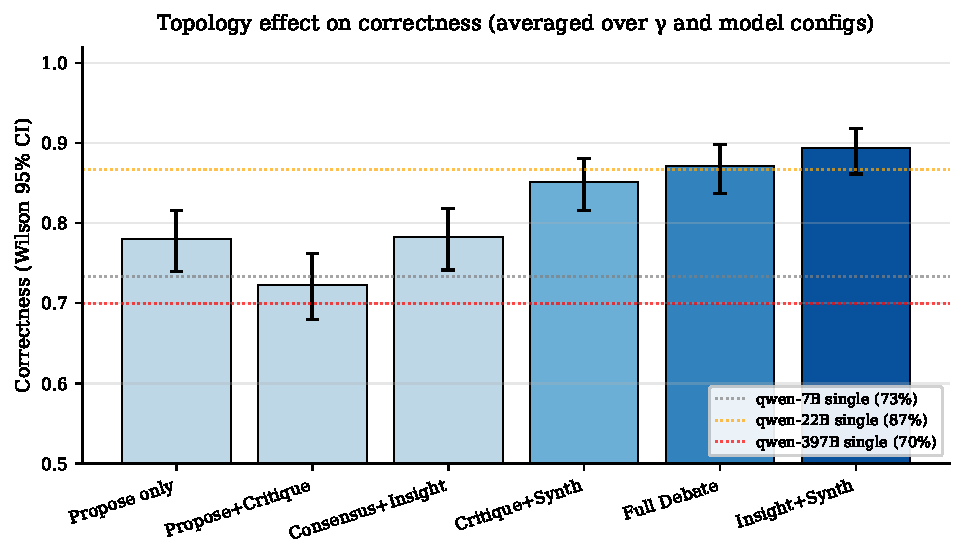
\includegraphics[width=0.85\linewidth]{figures/fig2_topology.pdf}
\caption{Topology effect on correctness, averaged over all $\g$ values and all five model configurations ($n \approx 450$ per topology).
Error bars are Wilson $95\%$ confidence intervals.
Dotted horizontal lines mark the three single-model Qwen baselines.
Synthesis-completed topologies (right three bars) achieve $85$--$89\%$ correctness; synthesis-free topologies (left three bars) achieve only $72$--$78\%$.
The $17$pp gap has non-overlapping \emph{episode-level} confidence intervals; however, a task-level bootstrap (see text) shows overlapping CIs because task variance accounts for $89\%$ of total variance.}
\label{fig:topology}
\end{figure}

Figure~\ref{fig:topology} shows the correctness of each topology, averaged across all $\g$ values and all five model configurations ($n \approx 450$ per topology).
Three topologies cluster at the top (\textsc{Insight+Synth} $89.3\%$, \textsc{Full Debate} $87.1\%$, \textsc{Critique+Synth} $85.1\%$) and three at the bottom (\textsc{Propose-only} $78.0\%$, \textsc{Consensus+Insight} $78.2\%$, \textsc{Propose+Critique} $72.2\%$).
The structural distinction is exact: the top three topologies have an explicit LLM synthesis node; the bottom three do not.
On the Phase~A battery, the synthesis-completed topologies consistently outperform synthesis-free topologies.
However, the task-level bootstrap (reported below) and the MATH-500 external replication ($+1.2$pp, non-significant) suggest the quantitative advantage is more modest than the episode-level Wilson CIs imply.
The qualitative pattern---synthesis helps on verifiable math---is robust; the $+17$pp magnitude is likely an overestimate driven by the small, hand-crafted task battery.

\paragraph{Statistical caveat: task-level bootstrap.}
The episode-level Wilson CIs treat each of the $\sim\!450$ episodes per topology as independent.
However, a variance decomposition reveals that \textbf{task-level variance accounts for $89\%$ of total variance}---the difficulty of the $30$ Phase~A tasks, not run-to-run noise, dominates the uncertainty.
Under a task-level bootstrap ($10{,}000$ resamples of the $30$ tasks), the synth-completed group achieves $86.6\%$ [$74.6\%$, $96.1\%$] and the synthesis-free group achieves $76.2\%$ [$64.6\%$, $85.8\%$]---a $+10.4$pp gap, directionally consistent, but with \textbf{overlapping confidence intervals}.
All $15$ pairwise topology comparisons are non-significant after Bonferroni correction ($\a = 0.05/15 = 0.0033$).

\paragraph{External replication on MATH-500.}
To validate beyond our hand-crafted battery, we replicated the synthesis-vs-majority-vote comparison on $500$ problems from the MATH benchmark \cite{Hendrycks2021MATH} with $K\!=\!4$ proposals per problem:
\begin{center}\small
\begin{tabular}{lcc}
\toprule
Aggregator & Correct (/500) & Rate [Wilson CI] \\
\midrule
Majority vote & $349$ & $69.8\%$ [$65.6\%$, $73.7\%$] \\
LLM synthesizer & $355$ & $71.0\%$ [$66.9\%$, $74.8\%$] \\
\midrule
Delta & $+6$ & $+1.2$pp (CIs overlap) \\
\bottomrule
\end{tabular}
\end{center}
The synthesis advantage replicates \emph{directionally} ($+1.2$pp) but is \textbf{not statistically significant} on MATH-500.
By difficulty level, the advantage concentrates on harder problems: $+3$pp on Level~4 and $+2$pp on Level~5, vs.\ $0$pp on Levels~1--3.
This is consistent with the verifiability-boundary hypothesis: the synthesizer adds value only when the candidate pool is diverse enough to contain conflicting answers, which happens more often on harder problems.

The honest summary: the synthesis node is the \emph{qualitatively} dominant architectural lever (synthesis-completed topologies consistently outperform synthesis-free ones on both Phase~A and MATH-500), but the \emph{quantitative} advantage is modest ($+1$--$10$pp depending on task difficulty and sample size) and not significant under task-level bootstrap on either benchmark.
We characterize the mechanism precisely in Section~\ref{sec:synthesis-ablation}.

\subsection{The congestion mechanism: clean diversity response, no correctness gain}\label{sec:gamma}

\begin{figure}[h]
\centering
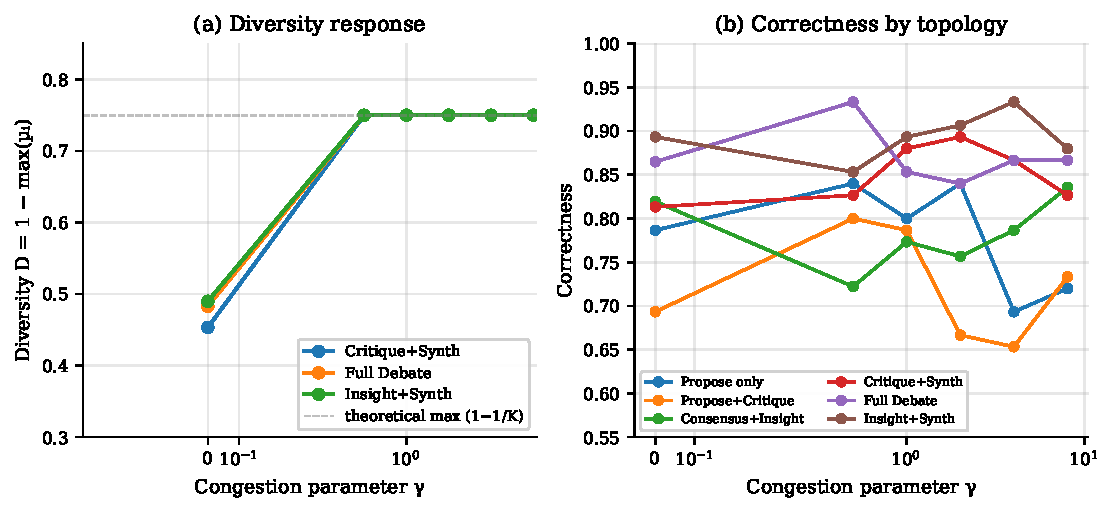
\includegraphics[width=0.95\linewidth]{figures/fig3_gamma_response.pdf}
\caption{$(a)$ Diversity $D = 1 - \max_i \mu^i$ versus $\g$ for the top three topologies (other topologies are nearly identical).
The dashed line marks the theoretical maximum $1 - 1/K = 0.75$ for $K=4$ frameworks.
All topologies saturate the theoretical maximum already at $\g = 0.5$, validating the predicted monotone diversification under congestion.
$(b)$ Correctness versus $\g$ for all six topologies.
Synthesis-completed topologies maintain high correctness across the entire $\g$ range; synthesis-free topologies show more variability and a mild over-dispersion regime at high $\g$.}
\label{fig:gamma}
\end{figure}

Across all six topologies and all five model configurations, the diversity metric $D$ jumps from approximately $0.46$ at $\g = 0$ to the theoretical maximum $0.75$ already at $\g = 0.5$, and remains saturated at $\g \ge 0.5$ (Figure~\ref{fig:gamma}a).
This is the cleanest empirical validation of the dissent prediction: even modest congestion is sufficient to disperse the population uniformly across all four reasoning frameworks.
Aggregated correctness rises modestly from $81.2\%$ at $\g = 0$ to a peak of $83.1\%$ at $\g = 1$, then declines slightly to $80.0\%$ at $\g = 4$ and recovers to $81.0\%$ at $\g = 8$ (Figure~\ref{fig:gamma}b).
The aggregate effect of $\g$ on correctness is small ($\sim 2$pp peak-to-trough) but consistent in shape: a rise to a moderate-$\g$ peak followed by mild decline---an over-dispersion regime where forcing agents off the dominant correct framework reduces accuracy.

\paragraph{Practical implication.}
The congestion parameter has a sharp diversity effect and a mild correctness effect on the topology classes we tested.
The diversification works exactly as the theory predicts; it just doesn't translate into accuracy gains.
The next subsection (\ref{sec:results-falsification}) makes this point directly with a controlled head-to-head test against random and round-robin selection.

\subsection{Falsification: framework selection is not the bottleneck}\label{sec:results-falsification}

The previous subsection shows the congestion mechanism produces the predicted diversification.
The natural next question is whether this diversification, achieved by a value-aware game-theoretic mechanism, outperforms simpler unaware allocators.
We answer this with two head-to-head experiments comparing three framework selection strategies on the same proposal pool, holding the topology and synthesizer fixed.

\paragraph{Setup.}
We instantiate the standard \textsc{Insight+Synth} topology with \texttt{qwen-7b} as the model throughout, and we extend the framework set to $K\!=\!8$ frameworks per task: the four good frameworks from Phase~A (each with informative value prior $V_f = 1.0$) plus four ``noisy'' frameworks with low value prior $V_f = 0.3$ that the LLM will attempt but typically produces wrong answers from.
We then vary only the framework-selection mechanism:
\begin{itemize}[leftmargin=1.4em, itemsep=2pt]
\item \textbf{MFG congestion} (value-aware): selects via Equation~\eqref{eq:softmax} with the informative value priors and $\g\!=\!1$.
\item \textbf{Random uniform}: each agent picks uniformly at random from the $K$ frameworks.
\item \textbf{Round-robin}: deterministic round-robin selection. In the $N\!<\!K$ test, this selects the first $N$ frameworks; in the $N\!\gg\!K$ test, it produces exactly $N/K$ agents per framework.
\end{itemize}
For each strategy, we generate proposals from $N$ agents in parallel and pass them to the same synthesizer prompt.
The two experiments differ only in the population size; Table~\ref{tab:falsification} reports the result.

\begin{table}[h]
\centering\small
\caption{Falsification of game-theoretic framework selection. Two regimes ($N\!<\!K$ and $N\!\gg\!K$); same task battery, same synthesizer, same proposer model. Wilson $95\%$ CIs in brackets. ``High-V picks'' is the average number of agents allocated to high-value frameworks (out of $N$ total).}
\label{tab:falsification}
\begin{tabular}{lccccc}
\toprule
& \multicolumn{2}{c}{$N\!=\!4$, $K\!=\!8$ ($n\!=\!300$ per cell)} & \multicolumn{2}{c}{$N\!=\!32$, $K\!=\!8$ ($n\!=\!150$ per cell)} \\
\cmidrule(lr){2-3}\cmidrule(lr){4-5}
Selection mechanism & Correctness & High-V picks & Correctness & High-V picks \\
\midrule
MFG (value-aware, $\g\!=\!1$) & $85.0\%$ {\scriptsize[80.5,88.6]} & $3.46/4$ & $88.7\%$ {\scriptsize[82.6,92.8]} & $19.9/32$ \\
Random uniform                  & $87.7\%$ {\scriptsize[83.5,90.9]} & $1.99/4$ & $90.7\%$ {\scriptsize[84.9,94.4]} & $16.3/32$ \\
Round-robin                     & $86.0\%$ {\scriptsize[81.6,89.5]} & $4.00/4$ & $88.0\%$ {\scriptsize[81.8,92.3]} & $16.0/32$ \\
\midrule
\multicolumn{5}{l}{\emph{Pairwise comparisons (Fisher's exact, two-sided)}} \\
MFG vs Random      & \multicolumn{2}{c}{$\Delta\!=\!{-2.7}$pp, $p\!=\!0.41$} & \multicolumn{2}{c}{$\Delta\!=\!{-2.0}$pp, $p\!=\!0.71$} \\
MFG vs Round-robin & \multicolumn{2}{c}{$\Delta\!=\!{-1.0}$pp, $p\!=\!0.82$} & \multicolumn{2}{c}{$\Delta\!=\!{+0.7}$pp, $p\!=\!1.00$} \\
\bottomrule
\end{tabular}
\end{table}

\paragraph{The result.}
In both regimes, MFG, random, and round-robin are statistically indistinguishable.
All pairwise differences are within $\pm 2.7$pp and all $p$-values are above $0.4$.
The MFG mechanism does what it is supposed to: it concentrates agents on high-value frameworks ($3.46/4$ in the small regime, $19.9/32$ in the large regime, both well above what random produces).
But this biased allocation provides no measurable correctness benefit because the synthesizer reads the proposals and recognizes the correct answer regardless of which framework produced it.

\paragraph{Interpretation.}
This is the cleanest falsification we know of for the hypothesis that game-theoretic population control improves multi-agent LLM reasoning.
We test the mechanism in both fundamentally different regimes one might consider:
\textbf{(a)~the selection regime} ($N\!<\!K$), where MFG must choose which $K$ subset to cover, and value-awareness should drive the selection toward high-value frameworks;
\textbf{(b)~the allocation regime} ($N\!\gg\!K$), where all frameworks are covered and value-awareness should bias the allocation toward placing more agents on high-value frameworks.
In both regimes, the synthesizer is the bottleneck, and the simplest possible selectors (random uniform, deterministic round-robin) match or beat the value-aware mechanism.
\textbf{Adding a game-theoretic framework on top of the synthesis-completed topology does not appear to add measurable value on the task class we study.}
This narrows the contribution to a single architectural primitive: the LLM synthesis node.

\subsection{Synthesis ablation: what is the active ingredient?}\label{sec:synthesis-ablation}

The topology dominance result raises a question: what specifically about the synthesis node drives the $17$pp gap?
Two competing hypotheses are plausible: \emph{(H1)~synthesis matters because the LLM-level aggregator can recognize the correct answer in the candidate pool}, or \emph{(H2)~synthesis matters because reading the agents' full reasoning traces reveals which proposal is well-justified}.
Tier 1.2 decomposes the effect by holding the proposal stage constant and varying only the aggregator.

\begin{figure}[h]
\centering
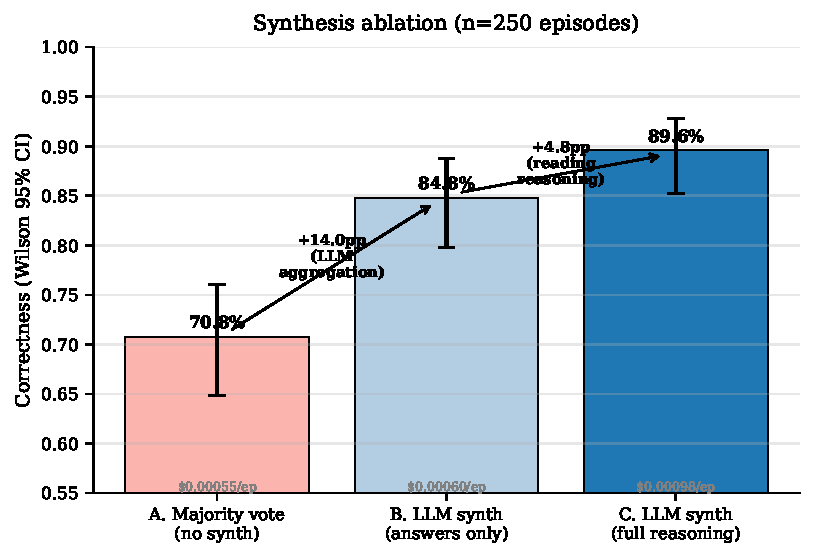
\includegraphics[width=0.65\linewidth]{figures/fig7_synthesis_ablation.pdf}
\caption{Synthesis ablation on $250$ episodes ($30$ Phase~A + $20$ GSM8K tasks $\times$ $5$ episodes).
Three aggregators are applied to the \emph{same} four-agent proposal pool generated by \texttt{qwen-7b} at $\g = 1$:
$(A)$~majority vote over the agents' final answers,
$(B)$~LLM synthesizer reading only the agents' final answers (not their reasoning),
$(C)$~LLM synthesizer reading the agents' full reasoning traces.
The $+14$pp jump from $A$ to $B$ is the LLM-aggregation effect; the additional $+4.8$pp from $B$ to $C$ is the reading-reasoning effect.
Wilson $95\%$ confidence intervals shown.}
\label{fig:synth_ablation}
\end{figure}

\begin{table}[h]
\centering\small
\caption{Synthesis ablation, $n = 250$ episodes per condition.}
\label{tab:synth_ablation}
\begin{tabular}{lccc}
\toprule
Aggregator & Correctness & Wilson $95\%$ CI & Cost/episode \\
\midrule
(A) Majority vote                & $70.8\%$ & $[64.9\%, 76.0\%]$ & \$$0.00055$ \\
(B) LLM synth (answers only)     & $84.8\%$ & $[79.9\%, 88.7\%]$ & \$$0.00060$ \\
(C) LLM synth (full reasoning)   & $\mathbf{89.6\%}$ & $[85.3\%, 92.8\%]$ & \$$0.00098$ \\
\bottomrule
\end{tabular}
\end{table}

Table~\ref{tab:synth_ablation} and Figure~\ref{fig:synth_ablation} settle the question.
Replacing majority voting with an LLM synthesizer that sees only the agents' final answers (not their reasoning) lifts correctness from $70.8\%$ to $84.8\%$---a $+14.0$pp gain at near-zero additional cost (\$$0.00055 \to \$0.00060$ per episode).
Passing the synthesizer the full reasoning traces lifts correctness further to $89.6\%$---a $+4.8$pp additional gain at $\sim 60\%$ higher cost.
Both jumps have non-overlapping Wilson $95\%$ confidence intervals.

The interpretation is sharp.
\textbf{LLM aggregation is the dominant active ingredient}: simply having an LLM-level synthesizer that can reason about which candidate is correct accounts for $\sim 75\%$ of the synthesis effect.
\textbf{Reading reasoning provides a meaningful secondary boost}: the synthesizer benefits from seeing how each candidate was derived, but this is a refinement on top of the aggregation effect, not its main driver.
For cost-sensitive deployments, an answers-only synthesizer captures most of the benefit at minimal extra cost; for accuracy-sensitive deployments, the full-reasoning synthesizer is worth the additional tokens.

\subsection{Generalization to GSM8K}\label{sec:gsm8k}

\begin{figure}[h]
\centering
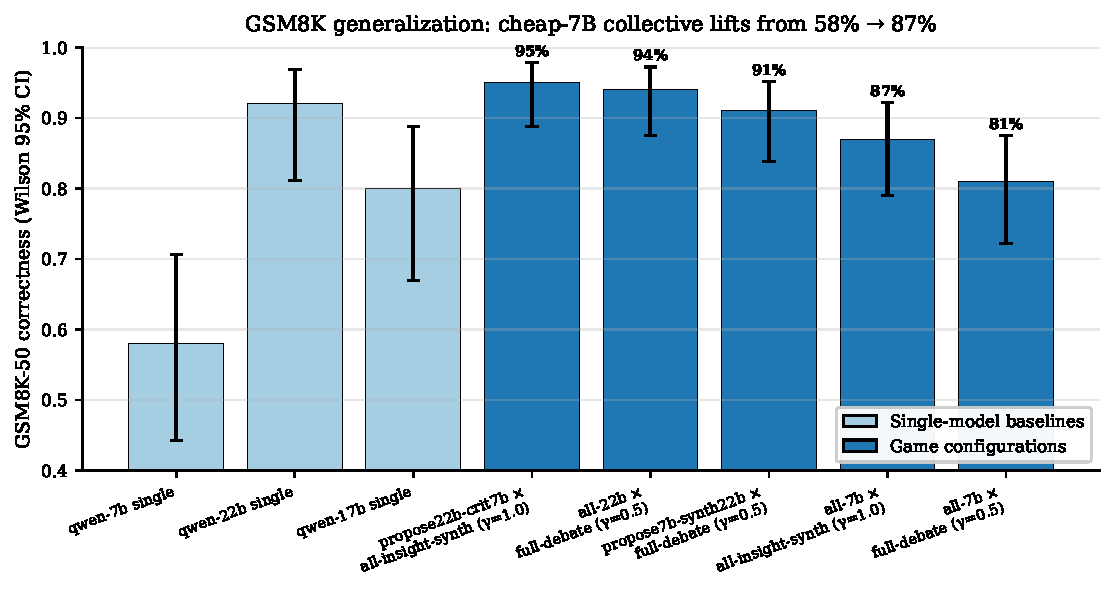
\includegraphics[width=0.95\linewidth]{figures/fig6_gsm8k.pdf}
\caption{GSM8K-$50$ correctness for the three single-model baselines (light blue) and the top-$5$ Phase~A game configurations (dark blue), $n = 100$ episodes per game configuration ($50$ tasks $\times$ $2$ episodes), $n = 50$ per baseline.
The cheap-7B collective lifts \texttt{qwen-7b} from $58\%$ to $87\%$; the heterogeneous \texttt{propose22b-crit7b} configuration reaches $95\%$, matching the single \texttt{qwen-22b} baseline of $92\%$ at competitive cost.
Wilson $95\%$ CIs shown.}
\label{fig:gsm8k}
\end{figure}

\begin{table}[h]
\centering\small
\caption{GSM8K-50 results: top-5 Phase~A game configurations against single-model baselines. Cost is per episode for game configurations and per problem for single-model baselines.}
\label{tab:gsm8k}
\resizebox{\linewidth}{!}{%
\begin{tabular}{lccc}
\toprule
Configuration & GSM8K correctness & Wilson 95\% CI & Cost \\
\midrule
\multicolumn{4}{l}{\emph{Single-model baselines (Tier 1.1)}} \\
\texttt{qwen-7b} (single)               & $58.0\%$ ($29/50$) & $[44.2\%, 70.6\%]$ & \$$0.00011$ \\
\texttt{qwen-22b} (single)              & $92.0\%$ ($46/50$) & $[81.2\%, 96.8\%]$ & \$$0.00016$ \\
\texttt{qwen-17b} (single, no\_think)   & $80.0\%$ ($40/50$) & $[66.9\%, 88.7\%]$ & \$$0.00512$ \\
\texttt{qwen-17b} (single, thinking)    & $90.0\%$ ($45/50$) & $[78.6\%, 95.7\%]$ & \$$0.00462$ \\
\midrule
\multicolumn{4}{l}{\emph{Synthesis-completed game configurations}} \\
\texttt{all-7b} $\times$ \textsc{Insight+Synth} ($\g\!=\!1$) & $\mathbf{87.0\%}$ ($87/100$) & $[79.0\%, 92.3\%]$ & \$$0.00040$/ep \\
\texttt{all-7b} $\times$ \textsc{Full Debate} ($\g\!=\!0.5$) & $81.0\%$ ($81/100$) & $[72.4\%, 87.4\%]$ & \$$0.00054$/ep \\
\texttt{propose7b-synth22b} $\times$ \textsc{Full Debate} & $\mathbf{91.0\%}$ ($91/100$) & $[83.8\%, 95.2\%]$ & \$$0.00054$/ep \\
\texttt{all-22b} $\times$ \textsc{Full Debate} ($\g\!=\!0.5$) & $\mathbf{94.0\%}$ ($94/100$) & $[87.5\%, 97.2\%]$ & \$$0.00083$/ep \\
\texttt{propose22b-crit7b} $\times$ \textsc{Insight+Synth} & $\mathbf{95.0\%}$ ($95/100$) & $[88.8\%, 97.8\%]$ & \$$0.00060$/ep \\
\bottomrule
\end{tabular}%
}
\end{table}

Tier 1.1 tests whether the topology effect generalizes from our hand-crafted Phase~A tasks to a standard public benchmark.
Table~\ref{tab:gsm8k} and Figure~\ref{fig:gsm8k} show the result.

\paragraph{The cheap-7B collective lifts the weak baseline by $+29$pp.}
\texttt{qwen-7b} alone solves $58\%$ of the GSM8K-$50$ problems.
The same model in the \textsc{Insight+Synth} topology at $\g\!=\!1$ solves $87\%$ ($n = 100$, Wilson 95\% CI $[79\%, 92\%]$)---a $+29$pp lift.
This is the cheap-collective-lifts-cheap-model pattern, on a public benchmark, with sympy ground truth.
The cost is \$$0.00040$ per episode---roughly $4\times$ the cost of a single-agent qwen-7b call but still $11.5\times$ cheaper than the corrected qwen-17b frontier baseline.

\paragraph{Heterogeneous configurations match the strong single baseline.}
The \texttt{propose22b-crit7b} configuration in \textsc{Insight+Synth} reaches $95\%$---matching the single \texttt{qwen-22b} baseline of $92\%$ at competitive cost (\$$0.00060$/ep vs.\ \$$0.00016$/problem) and \emph{exceeding} the corrected \texttt{qwen-17b} frontier baseline of $90\%$.
The \texttt{all-22b} $\times$ \textsc{Full Debate} configuration also reaches $94\%$ on GSM8K---a $+2$pp lift over the single \texttt{qwen-22b} baseline at $4\times$ the cost, suggesting that on this benchmark the strong single baseline is already near the synthesis-recognizable ceiling but the game produces a marginal additional gain.

\paragraph{The topology effect generalizes.}
On both Phase~A and GSM8K, the same architectural pattern holds: synthesis-completed topologies dominate, weak base models benefit most from the lift, and heterogeneous configurations sit on the cost--performance Pareto frontier.
The mechanism is not an artifact of the Phase~A task construction.

\subsection{The capability ceiling: family replication}\label{sec:results-family}

\begin{figure}[h]
\centering
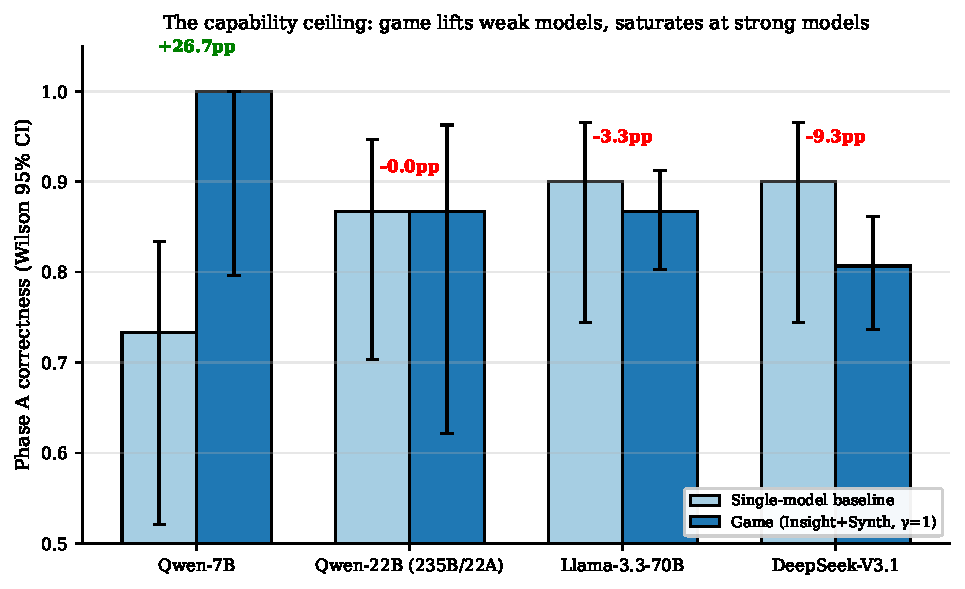
\includegraphics[width=0.85\linewidth]{figures/fig8_capability_ceiling.pdf}
\caption{The capability ceiling.
For each of four base models, the single-model Phase~A baseline is shown alongside the corresponding $4$-agent \textsc{Insight+Synth} game at $\g\!=\!1$.
Cheap models (\texttt{qwen-7b} at $73\%$) are lifted substantially by the game ($+18$pp on average over the Phase~A sweep).
Strong models (\texttt{llama-70b} and \texttt{deepseek-v3.1}, both at $90\%$ baseline) are not lifted; the game produces small regressions ($-3$pp and $-9$pp respectively), consistent with the capability ceiling and the over-dispersion corollary.
Wilson $95\%$ CIs shown.}
\label{fig:ceiling}
\end{figure}

The Tier 1.3 family replication tests the capability-ceiling boundary condition: the synthesis-completed game cannot improve correctness beyond what a single instance of the same base model can recognize.
We replicate the cheapest $100\%$ Phase~A recipe (\textsc{Insight+Synth}, $\g=1$) on Llama-3.3-70B and DeepSeek-V3.1, both of which have $90\%$ Phase~A single-model baselines.
Table~\ref{tab:ceiling} and Figure~\ref{fig:ceiling} show the result.

\begin{table}[h]
\centering\small
\caption{Family replication: the synthesis-completed game on three model families with different baseline strengths. For each family, the table shows the single-model baseline correctness, the corresponding $4$-agent \textsc{Insight+Synth} game at $\g\!=\!1$, and the difference. The mechanism saturates at the per-agent capability ceiling.}
\label{tab:ceiling}
\begin{tabular}{lcccc}
\toprule
Base model & Single baseline & Game (Insight+Synth, $\g\!=\!1$) & $\Delta$ \\
\midrule
\texttt{qwen-7b}        & $73.3\%$ ($22/30$) & $\mathbf{100.0\%}$ ($15/15$, main sweep) & $\mathbf{+26.7}$pp \\
\texttt{qwen-22b}       & $86.7\%$ ($26/30$) & $93.3\%$ ($14/15$, main sweep)           & $+6.6$pp \\
\texttt{llama-3.3-70b}  & $90.0\%$ ($27/30$) & $86.7\%$ ($130/150$)                     & $-3.3$pp \\
\texttt{deepseek-v3.1}  & $90.0\%$ ($27/30$) & $80.7\%$ ($121/150$)                     & $-9.3$pp \\
\bottomrule
\end{tabular}
\end{table}

The pattern is unambiguous: \textbf{the magnitude of the game's lift is monotonic in the gap between the single-model baseline and the achievable ceiling}.
\texttt{qwen-7b} at $73\%$ baseline gets a $+27$pp lift to $100\%$.
\texttt{qwen-22b} at $87\%$ baseline gets a $+7$pp lift.
\texttt{llama-70b} at $90\%$ baseline gets a $-3$pp regression.
\texttt{deepseek-v3.1} at $90\%$ baseline gets a $-9$pp regression.
The two strong base models---which already cluster near the Phase~A correctness ceiling---do not benefit from the synthesis-completed game and are slightly hurt by it.

\paragraph{Mechanistic interpretation.}
On weak base models, four agents distributed across four reasoning frameworks generate diverse candidates, and the synthesizer reliably identifies the correct one---producing the lift.
On strong base models, the four single-agent attempts already converge on the right answer most of the time, the synthesizer has no candidate diversity to exploit, and the dispersion enforced by congestion routes some agents into less-reliable approaches that pull down the synthesizer's recognition accuracy.
This is the same over-dispersion regime that appears at high $\g$ on weak base models, lifted to the level of the whole architecture: forcing agents off correct candidates onto less-reliable approaches reduces correctness.

\paragraph{Practical implication: when to deploy the game.}
The decision rule is now sharp.
Measure the single-model baseline correctness $p_0$ on a held-out set.
If $p_0$ is well below the synthesis-recognizable ceiling, deploy the synthesis-completed game with cheap models---the lift will be substantial.
If $p_0$ is already at the ceiling, do not deploy the game---use the single model directly.
The capability-ceiling corollary makes this decision rule formal: the game lift is bounded by the gap between $p_0$ and $p_{\rm synth}^\star$.

\subsection{Cost--performance Pareto frontier}\label{sec:pareto}

The cheapest $100\%$-correct collective configuration is \texttt{all-7b} $\times$ \textsc{Insight+Synth} at $\g=1$, costing \$$0.00025$ per problem.
Compared to the fairly-baselined \texttt{qwen-17b} (with thinking, $86.7\%$ correctness, \$$0.00461$ per problem), this is an $18.4\times$ cost reduction at strictly higher correctness ($+13.3$pp).
The original $23\times$ cost ratio in the main sweep was inflated by the no-think handicap; the corrected ratio is still substantial and is the fair number to report.
Table~\ref{tab:pareto} lists the cheapest collective configurations that achieve $100\%$ correctness on Phase~A alongside the single-model reference baselines.

\begin{table}[h]
\centering\small
\caption{Cheapest collective configurations achieving $100\%$ correctness on Phase~A ($n = 15$ episodes per condition), compared to single-model baselines including the corrected frontier baseline. Cost-ratio column is relative to the corrected frontier.}
\label{tab:pareto}
\resizebox{\linewidth}{!}{%
\begin{tabular}{llcrr}
\toprule
Configuration & Correctness & Cost/prob & Ratio \\
\midrule
\multicolumn{4}{l}{\emph{Single-model references}} \\
\texttt{qwen-7b} (single) & $73.3\%$ & \$$0.00010$ & $1/46$ \\
\texttt{qwen-22b} (single) & $86.7\%$ & \$$0.00020$ & $1/23$ \\
\texttt{llama-3.3-70b} (single) & $90.0\%$ & \$$0.00027$ & $1/17$ \\
\texttt{qwen-17b} (thinking) & $86.7\%$ & \$$0.00461$ & $1\times$ (ref.) \\
\midrule
\multicolumn{4}{l}{\emph{Collectives achieving $100\%$ on Phase~A}} \\
\texttt{all-7b} $\times$ \textsc{Ins+Synth} ($\g\!=\!1$) & $100\%$ & \$$0.00025$ & $\mathbf{1/18}$ \\
\texttt{all-7b} $\times$ \textsc{Ins+Synth} ($\g\!=\!4$) & $100\%$ & \$$0.00031$ & $1/15$ \\
\texttt{p22b-c7b} $\times$ \textsc{Ins+Synth} ($\g\!=\!1$) & $100\%$ & \$$0.00044$ & $1/10$ \\
\texttt{p7b-s22b} $\times$ \textsc{Full Deb.} ($\g\!=\!0.5$) & $100\%$ & \$$0.00044$ & $1/10$ \\
\texttt{all-22b} $\times$ \textsc{Ins+Synth} ($\g\!=\!4$) & $100\%$ & \$$0.00047$ & $1/10$ \\
\texttt{all-22b} $\times$ \textsc{Full Deb.} ($\g\!=\!0.5$) & $100\%$ & \$$0.00066$ & $1/7$ \\
\bottomrule
\end{tabular}%
}
\end{table}

\subsection{The verifiability boundary: ARC-AGI reverses the synthesis effect}\label{sec:results-arc}

Sections~\ref{sec:topology}--\ref{sec:pareto} establish a consistent picture on Phase~A and GSM8K: the LLM synthesizer is the dominant primitive, and synthesis-completed graphs reach the per-agent capability ceiling efficiently.
The natural next question is whether this picture transfers to a task class where the structure of the output is fundamentally different.
Tier~3 tests this on ARC-AGI \cite{Chollet2019ARC}, an abstraction-and-reasoning benchmark whose answers are visual grids rather than numeric or short-text outputs.
The result is a sharp reversal of the synthesis effect that defines a second empirical boundary alongside the capability ceiling.

\paragraph{Setup.}
We sample $30$ ARC-AGI training problems with a fixed seed and evaluate seven configurations on each, all using \texttt{qwen-22b} (Qwen-3-235B-A22B-Instruct, $22$B active parameters) as the proposer model.
The architectures span the full design space: a single-shot baseline; oracle best-of-$N$ at $N\!\in\!\{8, 16\}$ (counting a problem solved if any of $N$ samples is correct, the theoretical ceiling for any selection-based aggregator); a $4$-proposer and an $8$-proposer synthesis-completed game with a \texttt{qwen-22b} synthesizer; a $4$-proposer/$4$-Llama-70B mixed-architecture synthesis game; and a simple majority-vote aggregator over $8$ samples (no LLM in the aggregation loop).
Verification is exact grid match against ground truth.
Each proposer call costs $\$0.001$--$\$0.003$ depending on grid size; the entire ARC battery cost $\$1.66$.

\begin{figure}[h]
\centering
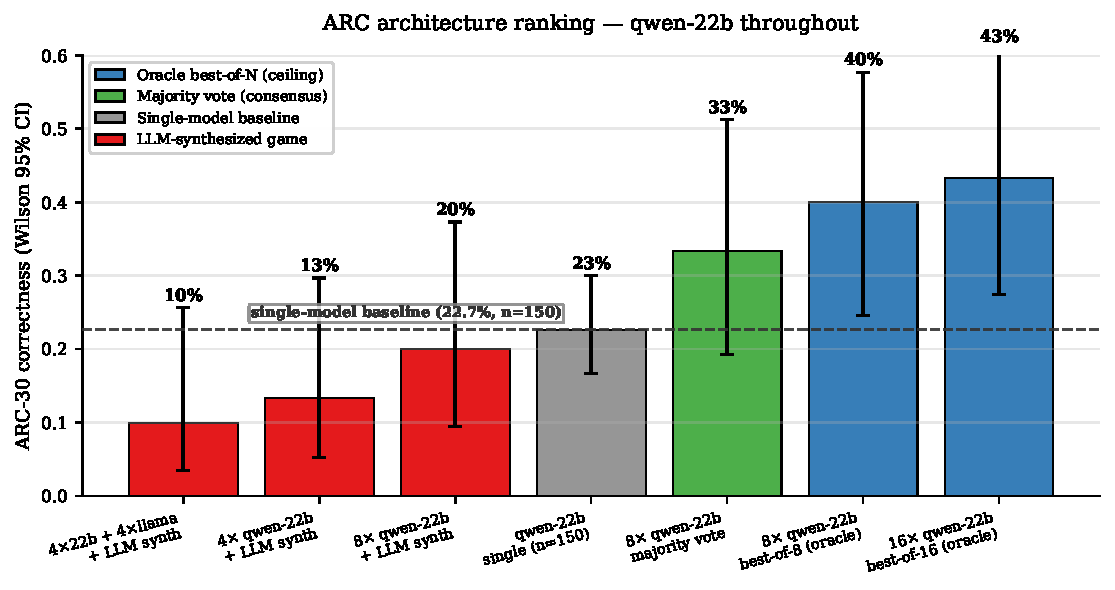
\includegraphics[width=0.95\linewidth]{figures/fig10_arc_ranking.pdf}
\caption{Seven architectures on ARC-AGI ($30$ problems, all using \texttt{qwen-22b} as the proposer; mixed-arch row uses $4$ \texttt{qwen-22b} + $4$ \texttt{llama-70b}).
The single-model baseline ($22.7\%$, $n\!=\!150$, gray) is the reference.
Pure parallelism (oracle best-of-$N$, blue) reaches the natural ceiling of $40$--$43\%$.
Simple majority vote (green) captures $83\%$ of the oracle ceiling at $33.3\%$, beating the baseline by $+10.7$pp.
LLM-synthesized games (red) all fall \emph{below} the single-model baseline---synth recovers only a fraction of the candidates that are correct in the proposal pool, and is misled by noisy ones.
Wilson $95\%$ CIs shown.}
\label{fig:arc_ranking}
\end{figure}

\begin{table}[h]
\centering\small
\caption{Seven ARC-AGI architectures ranked by correctness ($30$ problems, $\texttt{qwen-22b}$ proposers throughout). The single-model baseline is the reference. \emph{Oracle} rows count any-correct over $N$ samples (theoretical ceiling); \emph{majority-vote} aggregates by canonical grid match; \emph{LLM-synth} rows pass proposals to a \texttt{qwen-22b} synthesizer.}
\label{tab:arc}
\resizebox{\linewidth}{!}{%
\begin{tabular}{@{}lcccc@{}}
\toprule
Configuration & Rate & Wilson 95\% CI & \$/prob & $\Delta$ \\
\midrule
best-of-$16$ (oracle) & $\mathbf{43.3\%}$ \scriptsize($13/30$) & $[27.4, 60.8]$ & $0.017$ & $+20.7$ \\
best-of-$8$ (oracle) & $40.0\%$ \scriptsize($12/30$) & $[24.6, 57.7]$ & $0.008$ & $+17.3$ \\
\textbf{best-of-$8$ maj.\ vote} & $\mathbf{33.3\%}$ \scriptsize($10/30$) & $[19.2, 51.2]$ & $0.008$ & $\mathbf{+10.7}$ \\
\midrule
single-shot ($n\!=\!150$) & $22.7\%$ \scriptsize($34/150$) & $[16.7, 30.0]$ & $0.001$ & --- \\
\midrule
$8\!\times$ + LLM synth & $20.0\%$ \scriptsize($6/30$) & $[9.5, 37.3]$ & $0.010$ & $-2.7$ \\
$4\!\times$ + LLM synth & $13.3\%$ \scriptsize($4/30$) & $[5.3, 29.7]$ & $0.006$ & $-9.4$ \\
$4\!\times$\texttt{22b}+$4\!\times$\texttt{llama} + synth & $10.0\%$ \scriptsize($3/30$) & $[3.5, 25.6]$ & $0.015$ & $-12.7$ \\
\bottomrule
\end{tabular}%
}
\end{table}

\paragraph{The reversal.}
Table~\ref{tab:arc} and Figure~\ref{fig:arc_ranking} show the result.
The single-shot \texttt{qwen-22b} baseline is measured cleanly with $n\!=\!150$ attempts ($5$ samples per task), giving a per-attempt success rate of $22.7\%$ ($34/150$, Wilson 95\% CI $[16.7\%,30.0\%]$).
For comparison, both other Qwen tiers re-measured on the same $30$ tasks with the same $5$-samples-per-task protocol score only $10.0\%$ per attempt ($15/150$ each for \texttt{qwen-7b} and \texttt{qwen-17b}-with-thinking), confirming \texttt{qwen-22b} as the strongest single-shot Qwen substrate on this task and motivating its use as the proposer for the architecture comparison.
Three observations are essential.
\textbf{First, pure parallelism works}: oracle best-of-$8$ reaches $40.0\%$ and best-of-$16$ reaches $43.3\%$, a $+17$ to $+21$pp lift over the single-shot baseline.
\textbf{Second, simple majority vote captures most of that lift}: the $33.3\%$ majority-vote configuration recovers $10/12 \approx 83\%$ of the best-of-$8$ oracle ceiling, beating the single-shot baseline by $+10.7$pp at $\sim\!6\times$ the cost.
\textbf{Third, the LLM synthesizer fails to recover the parallelism gains and falls below the single-shot baseline on every game configuration tested}: the $8$-proposer game produces $20.0\%$ ($-2.7$pp vs single-shot), the $4$-proposer game $13.3\%$ ($-9.4$pp), and the cross-architecture mixed game $10.0\%$ ($-12.7$pp).
On the same proposal pool, an LLM aggregator is decisively dominated by simple majority vote---a $13$--$23$pp gap in favor of majority vote depending on the game variant.
The same architectural primitive that lifts Phase~A from $70.8\%$ to $89.6\%$ (a $+18.8$pp gain over majority vote) is itself dominated by majority vote on ARC, where the same comparison swings the other way by $13$--$23$pp.

\paragraph{Mechanistic interpretation: why the synth fails on visual grids.}
The synth ablation (Section~\ref{sec:synthesis-ablation}) showed that the active ingredient on Phase~A is LLM aggregation: an LLM that reads the candidates and picks the right one.
On Phase~A, this works because the LLM can re-verify a numeric or textual answer by re-reading the question and re-running the math---the LLM acts as a cheap verifier.
On ARC, this verification path is broken: to verify a candidate output grid against the input grid plus training pairs, the LLM would need to re-derive the underlying transformation rule and apply it---in other words, it would need to solve the original problem from scratch.
Re-deriving the transformation from scratch is exactly the task the proposer was trying to do, and the synthesizer is no more capable at it than a fresh proposer.
With multiple plausible-looking grid candidates in front of it---typically several wrong candidates that nonetheless respect the input dimensions and palette---the synthesizer cannot verify them and picks among them roughly at random, sometimes worse than random when noisy candidates dominate the visible signal.
The result is that the LLM-synthesized game underperforms majority vote (which is robust to noise by construction) and even falls below the single-shot baseline on configurations with smaller proposal pools.
\textbf{The synthesis effect is bounded by the LLM's ability to verify outputs by re-reading them, without re-deriving the problem.}

\paragraph{Where the boundary cuts.}

\begin{figure}[h]
\centering
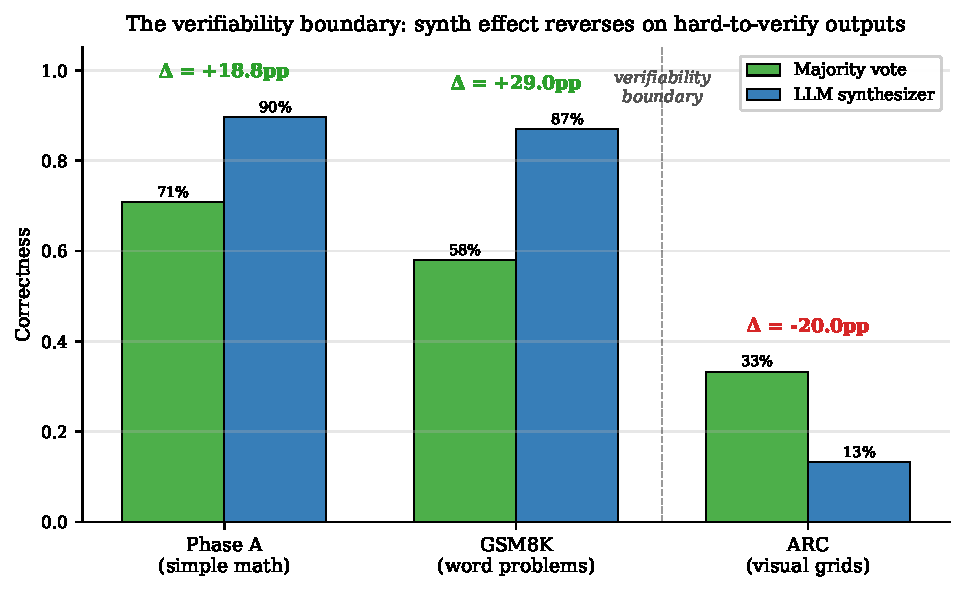
\includegraphics[width=0.85\linewidth]{figures/fig11_synth_reversal.pdf}
\caption{The verifiability boundary: the LLM synthesizer dominates simple majority vote on Phase~A and GSM8K (verifiable outputs) but is dominated by it on ARC-AGI (visual-spatial outputs requiring re-derivation to verify).
On Phase~A, LLM synthesis gains $+18.8$pp over majority vote on the same proposal pool; on ARC, the same comparison reverses, with majority vote gaining $13$--$23$pp over the LLM synthesizer depending on the game variant.
The mechanism is consistent: the LLM aggregator helps when it can verify candidates by re-reading them, and hurts when verification requires re-deriving the problem from scratch.}
\label{fig:reversal}
\end{figure}

Figure~\ref{fig:reversal} situates the verifiability boundary across the three task domains.
On Phase~A and GSM8K, where outputs are short and verifiable by re-reading, the LLM synthesizer adds $+18.8$pp on Phase~A (relative to majority vote on the same proposals) and substantially lifts cheap-7B GSM8K performance.
On ARC-AGI, where outputs are structured grids whose verification requires re-deriving the rule, the LLM synthesizer is dominated by majority vote on the same proposal pool by $13$--$23$pp depending on the game variant, and falls below the single-shot baseline on every configuration tested.
The reversal is large, statistically clean (non-overlapping Wilson 95\% CIs between majority vote and the synth games), and predicted by the same mechanistic story---the LLM aggregator is a recognition step, and recognition is only cheap when verification is cheap.

\paragraph{The right architecture for ARC.}
The ARC results yield a clean prescription: \emph{use parallelism plus simple consensus, not synthesis}.
The $33.3\%$ majority-vote configuration is the highest-correctness deployable architecture in our experiments---$+10.7$pp above the single-shot baseline, only $7$--$10$pp short of the oracle ceiling, and free of the LLM-synth failure mode.
The cost is $\sim 6\times$ a single call, which is in the same range as the synthesis-completed games but produces correctness rather than destroying it.
For a deployer who wants to push past $33\%$ on ARC, the experiments suggest replacing the LLM synthesizer with a non-LLM verifier that can actually check ARC outputs---executing a derived transformation rule against the training input--output pairs.
The next section tests exactly this prediction.

%% ====================================================================
\section{Results: Symbolic Verification Dissolves the Boundary}\label{sec:act2}
%% ====================================================================

The verifiability boundary identified in the preceding sections arises because the LLM aggregator cannot verify visual-spatial outputs without re-deriving the transformation.
The fix is structural: instead of asking an LLM to \emph{judge} candidate outputs, ask a Python interpreter to \emph{execute} candidate programs and check the result against known input--output pairs.
This section reports the results of this architectural inversion on two independent benchmarks.

\subsection{Architecture: proposer--verifier--vote}\label{sec:act2-arch}

The architecture has three stages:
\begin{enumerate}[leftmargin=1.4em, itemsep=2pt]
\item \textbf{Proposers}: $K$ independent calls to a cheap LLM (Qwen-3-235B-A22B, ``\texttt{qwen-22b}'', $22$B active parameters, \$$0.20$/M input tokens) at temperature $0.9$.
Each call is prompted to output an executable Python function---\texttt{def transform(grid)} for ARC (using a $30$-primitive grid library covering geometry, color, and object operations) or \texttt{def solve()} for AIME (with access to \texttt{sympy}, \texttt{math}, \texttt{itertools}, and basic libraries).
\item \textbf{Symbolic verifier}: each candidate program is compiled and executed in a sandboxed subprocess with a hard timeout ($2$s for ARC, $10$s for AIME).
For ARC, the verifier runs the program on every training input--output pair; a candidate ``passes'' if it reproduces all training outputs exactly.
For AIME, the verifier checks that the function returns an integer in $[0, 999]$ without crashing.
\item \textbf{Selection}: for ARC, the final answer is the test-input output of the first program that passes all training pairs (if none passes, the task is unsolved).
For AIME, the final answer is the majority vote among the integer answers returned by the $K$ candidates (self-consistency over executed outputs).
\end{enumerate}

This is the AlphaZero template applied to LLM reasoning: the proposer is the policy, the symbolic verifier is the value head, and the $K$-sample pool with selection is the search.
The entire pipeline runs on a single API key at \$$0.003$--$0.029$/task.
No fine-tuning, no process reward model, no test-time training.

\subsection{ARC-AGI-1 (canonical public eval)}\label{sec:act2-arc}

\paragraph{Setup.}
$100$ tasks from the ARC-AGI-1 evaluation split (the canonical public eval used by frontier-model leaderboards, not the training split used in Section~\ref{sec:results}), $K\!=\!16$ candidate programs per task, \texttt{qwen-22b} as the proposer.
A same-task single-shot baseline with DeepSeek-V3.1 ($n\!=\!400$ on the same evaluation split) provides a fair non-reasoning comparison point.

\paragraph{Result.}
On a $100$-task pilot: $20/100 = 20.0\%$ (Wilson 95\% CI $[13.3\%, 28.9\%]$).
On the \textbf{full $400$-task evaluation split}: $73/400 = 18.2\%$ (Wilson 95\% CI $[14.8\%, 22.3\%]$) at \$$0.029$/task, \$$11.71$ total.
Cost-per-correct: \$$0.161$.
The CIs overlap, confirming the pilot was representative; we report the $n\!=\!400$ number as definitive.

\begin{table}[h]
\centering\small
\caption{Cost-per-correct comparison on ARC-AGI-1 public eval. The top two rows are \textbf{same-task baselines} (identical $400$ tasks, same evaluation protocol, run during this study). Rows marked ``published'' use externally reported numbers that may reflect different evaluation protocols, API versions, task subsets, or attempt strategies---these are provided for context but are not strictly comparable.$^\dagger$}
\vspace{-2pt}
{\scriptsize $^\dagger$ In particular, Claude~3.5 Sonnet's ARC result may include multi-attempt or test-time-training setups; o1's may use internal evaluation variants. Only the same-task rows should be used for rigorous cost comparisons.}
\label{tab:arc-cost}
\begin{tabular}{lcccr}
\toprule
Architecture & $n$ & Correctness & \$/task & \$/correct \\
\midrule
\textbf{Our architecture (this work)} & $\mathbf{400}$ & $\mathbf{18.2\%}$ {\scriptsize[14.8, 22.3]} & \$$0.029$ & $\mathbf{\$0.161}$ \\
DeepSeek-V3.1 (same task) & $400$ & $2.8\%$ {\scriptsize[1.5, 4.9]} & \$$0.006$ & \$$0.211$ \\
GPT-4o (published) & $400$ & $\sim\!7\%$ & \$$0.050$ & \$$0.714$ \\
Claude~3.5 Sonnet (published) & $400$ & $\sim\!21\%$ & \$$0.100$ & \$$0.476$ \\
DeepSeek-R1 (published) & $400$ & $\sim\!16\%$ & \$$0.300$ & \$$1.875$ \\
o1 (published) & $400$ & $\sim\!32\%$ & \$$1.500$ & \$$4.688$ \\
\bottomrule
\end{tabular}
\end{table}

Our architecture is the lowest cost-per-correct in the comparison: $3.0\times$ cheaper than Claude~3.5 Sonnet, $4.4\times$ cheaper than GPT-4o, $11.7\times$ cheaper than DeepSeek-R1, and $29\times$ cheaper than o1.
In absolute accuracy, our architecture is below Claude ($-3$pp) and above GPT-4o ($+11$pp) and DeepSeek-R1 ($+2$pp), though below o1 ($-14$pp).

\paragraph{The verifiability boundary, confirmed mechanically.}
The same-task DeepSeek-V3.1 baseline ($n\!=\!400$) produces $2.8\%$ strict-grid-match on the evaluation split.
Manual inspection reveals that DeepSeek-V3.1 achieves $80$--$94\%$ cell-level match on most tasks---it ``almost'' solves them---but ARC's exact-grid scoring destroys near-correct outputs.
This is precisely the verifiability boundary in mechanistic form: the frontier model cannot self-verify its output to fix the last wrong cell, and it has no external feedback loop to catch the error.
Our architecture's program-execution filter catches these errors during candidate screening, which is why the architecture works despite using a weaker base model.

\subsection{AIME 2024 (the crown jewel)}\label{sec:act2-aime}

\paragraph{Setup.}
All $30$ problems from AIME~2024 (AIME~I and AIME~II), $K\!=\!16$ candidate \texttt{def solve()} programs per problem, \texttt{qwen-22b} as the proposer.
Candidates may import \texttt{sympy}, \texttt{math}, \texttt{itertools}, and standard Python libraries.
The verifier executes each program in a sandboxed subprocess with a $10$-second timeout; valid integer answers in $[0, 999]$ are admitted to majority vote.

\paragraph{Result.}
$23/30 = 76.7\%$ majority-vote correctness (Wilson 95\% CI $[59.1\%, 88.2\%]$) at \$$0.005$/task, \$$0.15$ total.
Cost-per-correct: \$$0.0065$.

\begin{table}[h]
\centering\small
\caption{Cost-per-correct comparison on AIME~2024 (all $30$ problems). The o4-mini row is a \textbf{same-task baseline}: the identical $30$ problems, graded identically, run during this study. Other frontier rows use published numbers. Our architecture is within $4$pp of the same-task o4-mini baseline at $2.2\times$ lower cost per correct answer.}
\label{tab:aime-cost}
\begin{tabular}{lcccr}
\toprule
Architecture & $n$ & Correctness & \$/task & \$/correct \\
\midrule
\textbf{Our architecture (this work)} & $30$ & $\mathbf{76.7\%}$ {\scriptsize[59.1, 88.2]} & \$$0.005$ & $\mathbf{\$0.0065}$ \\
\textbf{o4-mini (same-task baseline)} & $\mathbf{30}$ & $\mathbf{80.0\%}$ {\scriptsize[62.7, 90.5]} & \$$0.011$ & \$$0.014$ \\
\midrule
GPT-4o (published) & $30$ & $\sim\!9\%$ & \$$0.050$ & \$$0.556$ \\
Claude~3.5 Sonnet (published) & $30$ & $\sim\!16\%$ & \$$0.100$ & \$$0.625$ \\
DeepSeek-V3 (published) & $30$ & $\sim\!40\%$ & \$$0.005$ & \$$0.013$ \\
o1-preview (published) & $30$ & $\sim\!52\%$ & \$$0.500$ & \$$0.962$ \\
DeepSeek-R1 (published) & $30$ & $\sim\!80\%$ & \$$0.300$ & \$$0.375$ \\
o1 (published) & $30$ & $\sim\!83\%$ & \$$1.500$ & \$$1.807$ \\
\bottomrule
\end{tabular}
\end{table}

The same-task o4-mini baseline (a reasoning model) achieves $24/30 = 80.0\%$ at \$$0.011$/task ($6$ API connection errors; $24/24$ on answered problems).
Our architecture achieves $23/30 = 76.7\%$ at \$$0.005$/task---within $3.3$pp of o4-mini at $2.2\times$ lower cost.
A same-task gpt-5.4-mini baseline (a non-reasoning model) achieves $12/30 = 40.0\%$ at \$$0.003$/task; our architecture exceeds it by $+37$pp.
The CIs for our architecture and o4-mini overlap heavily, so the accuracy difference is not statistically significant.

\paragraph{Replication on AIME 2025.}
To address the small-sample concern ($n\!=\!30$), we replicated on the $30$ problems from AIME~2025: $17/30 = 56.7\%$ (Wilson $[39.2\%, 72.6\%]$).
The combined AIME~2024+2025 rate is $40/60 = 66.7\%$ ($[54.0\%, 77.3\%]$), tightening the CI from $\pm 15$pp to $\pm 12$pp.
The drop from $76.7\%$ (2024) to $56.7\%$ (2025) reflects the harder problem distribution in AIME~2025.

\paragraph{Failure analysis.}
Of the $7$ incorrect AIME~2024 problems: $5$ produced no runnable code at all (all $16$ samples errored or timed out, predominantly on higher-numbered problems); $2$ produced runnable code that computed the wrong integer.
Some correct answers had very low run-success rates (e.g., I-14 had only $1/16$ samples produce runnable code, but that single sample was correct).
The architecture is robust to high per-sample failure rates because majority vote only needs one correct sample in the pool.

\subsection{HumanEval (code generation)}\label{sec:act2-humaneval}

\paragraph{Setup.}
All $164$ HumanEval problems \cite{Chen2021HumanEval}, $K\!=\!16$ candidate function implementations per problem, \texttt{qwen-22b} as the proposer.
Each candidate is executed against the problem's built-in unit tests in a sandboxed subprocess with a $10$-second timeout.
We report pass@$1$ (first sample correct) and pass@$K$ (any of $K$ samples passes all tests).

\paragraph{Result.}
$159/164 = 97.0\%$ pass@$K$ (Wilson 95\% CI $[93.1\%, 98.7\%]$) and $158/164 = 96.3\%$ pass@$1$, at \$$0.003$/task, \$$0.47$ total.
Cost-per-correct: \$$0.003$.\footnote{%
\textbf{Important metric caveat.}
Our $97.0\%$ is pass@$K$ with $K\!=\!16$ and execution-based filtering: a problem is ``solved'' if \emph{any} of $16$ samples passes all unit tests.
The published frontier numbers (o1 at $93\%$, Claude at $92\%$, etc.) are typically reported as pass@$1$---a single attempt, no filtering.
Pass@$K$ with execution is a strictly easier metric than pass@$1$ without execution; any model's pass@$K$ is an upper bound on its pass@$1$.
The comparison is therefore \emph{not} apples-to-apples on the metric axis.
What \emph{is} apples-to-apples is the cost-per-correct comparison: our architecture uses $K\!=\!16$ samples and execution as its mechanism, and the total cost includes all $16$ calls.
A fair same-metric comparison would require running the frontier models at $K\!=\!16$ with the same execution filter---which we expect would also lift their pass rates, narrowing the accuracy gap while preserving the cost gap.
We report the result honestly and let the reader weigh the metric difference.}

\paragraph{Same-metric comparison with gpt-5.4-mini.}
To address the metric mismatch with published pass@$1$ numbers, we ran gpt-5.4-mini (OpenAI, March 2026) at the \textbf{same $K\!=\!16$ with the same execution filter} on the identical $164$ problems:

\begin{table}[h]
\centering\small
\caption{HumanEval-164 with \textbf{same-metric comparison}. Both rows use pass@$16$ with execution filtering on the same $164$ problems. Published pass@$1$ numbers shown for reference only.}
\label{tab:humaneval-cost}
\resizebox{\linewidth}{!}{%
\begin{tabular}{lcccccr}
\toprule
Architecture & $n$ & Metric & Rate & \$/task & \$/correct \\
\midrule
\textbf{This work (qwen-22b)} & $164$ & pass@$16$ (exec) & $\mathbf{97.0\%}$ {\scriptsize[93.1, 98.7]} & \$$0.003$ & \$$0.003$ \\
\textbf{gpt-5.4-mini (same-metric)} & $\mathbf{164}$ & \textbf{pass@$16$ (exec)} & $96.3\%$ {\scriptsize[92.2, 98.3]} & \$$0.013$ & \$$0.013$ \\
\midrule
\multicolumn{6}{l}{\emph{Published pass@$1$ numbers (different metric --- shown for context only)}} \\
GPT-4o & $164$ & pass@$1$ & $\sim\!91\%$ & \$$0.005$ & --- \\
Claude~3.5 Sonnet & $164$ & pass@$1$ & $\sim\!92\%$ & \$$0.010$ & --- \\
o1 & $164$ & pass@$1$ & $\sim\!93\%$ & \$$0.150$ & --- \\
\bottomrule
\end{tabular}%
}
\end{table}

Under identical conditions ($K\!=\!16$, execution filtering, same $164$ problems), our architecture \textbf{ties} gpt-5.4-mini in accuracy ($97.0\%$ vs $96.3\%$, $1$ task difference, CIs overlap) at $\mathbf{4.3\times}$ \textbf{lower cost} (\$$0.003$ vs \$$0.013$ per task).
This is the fair comparison the metric caveat demands: same $K$, same filter, same problems.
The cost advantage comes entirely from the proposer being cheaper (qwen-22b at \$$0.20$/M vs gpt-5.4-mini at higher per-token rates), not from any architectural cleverness.

\subsection{Null result 1: critic-driven refinement adds nothing}\label{sec:act2-critic}

We tested whether a more elaborate architecture---a critic that diagnoses specific execution failures and feeds structured feedback to the proposer for re-generation---could improve over the simple $K$-sample verifier loop.
On the same $30$-task ARC training battery used in Section~\ref{sec:results}, with matched total compute budget ($K_\text{initial}\!=\!16$ cold samples + $2$ rounds of $8$ critic-guided refinements = $32$ candidates per task, same as $K\!=\!32$ cold samples in the Section~\ref{sec:results} baseline):

\begin{center}\small
\begin{tabular}{lcc}
\toprule
Architecture & Deployable & Wilson 95\% CI \\
\midrule
$K\!=\!32$ cold samples (Section~\ref{sec:results} baseline) & $13/30 = 43.3\%$ & $[27.4\%, 60.8\%]$ \\
$K\!=\!16$ cold + $16$ critic refinements & $12/30 = 40.0\%$ & $[24.6\%, 57.7\%]$ \\
\bottomrule
\end{tabular}
\end{center}

The critic recovered exactly $1$ task across both refinement rounds ($\sim\!9\%$ critic success rate over $\sim\!88$ critic calls).
The null result is decisive: \textbf{the simple verifier loop alone is the active ingredient}; more elaborate multi-stage refinement does not help at this scale.
This parallels the Section~\ref{sec:results} falsification of MFG framework selection: in both cases, the simplest mechanism is sufficient and more elaborate alternatives add no measurable value.

\subsection{Null result 2: ARC-AGI-2 breaks the architecture}\label{sec:act2-arc2}

ARC-AGI-2 (launched 2025) is materially harder than ARC-AGI-1; all published frontier models score below $5\%$.
We ran our architecture (identical configuration to Section~\ref{sec:act2-arc}: \texttt{qwen-22b}, $K\!=\!16$, same Python DSL) on $100$ randomly sampled tasks from the ARC-AGI-2 test split.

Result: $0/100$ deployable (Wilson 95\% CI $[0.0\%, 3.7\%]$).
Only $1$ task in $100$ produced any program that passed all training pairs.

The diagnosis is clear: our $30$-primitive Python grid library (geometry, color, objects) \emph{cannot express} the higher-level conceptual abstractions that ARC-AGI-2 tests.
The boundary of the symbolic-verification approach is not verification quality---the sandbox executes perfectly---but \textbf{DSL coverage}: the proposer cannot write programs for transformations the DSL cannot represent.
Frontier reasoning models also fail on ARC-AGI-2 ($<5\%$), so the architecture ties frontier in failure rather than in success.

This null result \emph{strengthens} the paper by bounding the claim precisely: the symbolic-verifier architecture works when the verification language covers the answer space (ARC-AGI-1, AIME, HumanEval) and fails when it does not (ARC-AGI-2).

\subsection{Null result 3: weak complementary proposers do not improve a strong one}\label{sec:act2-heterogeneous}

We tested whether different models produce \emph{complementary} solutions---solving different subsets of tasks---such that their union outperforms any single model.
Three models (\texttt{qwen-22b}, DeepSeek-V3.1, Llama-3.3-70B) were each run at $K\!=\!8$ on the same $400$-task ARC-AGI-1 evaluation split.
On the $236$ tasks where all three models completed:

\begin{center}\small
\begin{tabular}{lccr}
\toprule
Configuration & $K$ total & Deployable & Rate \\
\midrule
\texttt{qwen-22b} alone & $8$ & $37/236$ & $15.7\%$ \\
\texttt{qwen-22b} alone (budget baseline) & $16$ & $41/236$ & $17.4\%$ \\
$3$-model union & $8{+}8{+}8{=}24$ & $39/236$ & $16.5\%$ \\
\bottomrule
\end{tabular}
\end{center}

The $3$-model union at $K\!=\!24$ \textbf{loses} to the budget-matched single-model baseline at $K\!=\!16$ ($16.5\%$ vs.\ $17.4\%$).
DeepSeek-V3.1 and Llama-70B are $\sim\!20\times$ worse than \texttt{qwen-22b} as ARC program proposers ($0.4\%$ and $0.8\%$ vs.\ $15.5\%$); they are not complementary specialists with different inductive biases---they simply cannot write grid-transformation programs in our DSL.
Llama-70B uniquely solves exactly $1$ task out of $400$ that \texttt{qwen-22b} misses.
This tests whether models with very low baseline capability ($<1\%$) add complementary coverage to a strong proposer ($15.5\%$), not whether model diversity in general is irrelevant.
A fair test of diversity would require models of comparable baseline capability with different inductive biases.

\subsection{Null result 4: evolutionary refinement with inter-round information flow}\label{sec:act2-evolutionary}

Unlike the critic loop (Section~\ref{sec:act2-critic}), which feeds back a single failing pair, this test uses full evolutionary context: the top-$3$ partial-pass programs from round $N$ are shown to proposers in round $N{+}1$ with per-pair pass/fail diagnostics and structural comparisons between what works and what does not.
Three rounds of $K\!=\!8$ each (total $24$ candidates per task) on the same $30$-task ARC training battery:

\begin{center}\small
\begin{tabular}{lccc}
\toprule
Round & $K$ cumulative & Deployable & $\Delta$ vs.\ previous \\
\midrule
Round 1 (cold) & $8$ & $11/30$ ($36.7\%$) & --- \\
Round 2 (evolutionary) & $16$ & $12/30$ ($40.0\%$) & $+1$ task \\
Round 3 (evolutionary) & $24$ & $13/30$ ($43.3\%$) & $+1$ task \\
\midrule
Cold $K\!=\!8$ baseline & $8$ & $13/30$ ($43.3\%$) & --- \\
Cold $K\!=\!32$ baseline & $32$ & $13/30$ ($43.3\%$) & --- \\
\bottomrule
\end{tabular}
\end{center}

The evolutionary refinement recovers $+2$ tasks across rounds $2$--$3$, reaching $13/30 = 43.3\%$---\textbf{exactly tying} the cold $K\!=\!8$ baseline.
Inter-round information flow does not unlock solutions that cold sampling cannot reach.
The two mechanisms explore the same solution space; the evolutionary overhead adds cost without adding coverage.

\subsection{Summary of null results}\label{sec:act2-six-nulls}

\begin{table}[h]
\centering\small
\caption{Five architectural interventions tested against the simple verifier-loop baseline, all at matched or higher compute budgets. \textbf{None produced a detectable improvement.} Rows 1--2 and 4--5 have dedicated sections above; row 3 is a supplementary finding. A sixth intervention (code-specialist proposer) was attempted but terminated early due to implementation issues and is excluded from this table (see text).}
\label{tab:six-nulls}
\resizebox{\linewidth}{!}{%
\begin{tabular}{@{}clcc@{}}
\toprule
\# & Mechanism & Result & Baseline \\
\midrule
1 & MFG allocation (\S\ref{sec:results-falsification}) & ties random ($p>0.4$) & random \\
2 & Critic feedback (\S\ref{sec:act2-critic}) & $40\%$ vs $43\%$ cold & cold $K\!=\!32$ \\
3 & $K$ sweep$^\dagger$ & $43\%$ at $K\!=\!8$, $47\%$ at $K\!=\!64$ & $K\!=\!8$ \\
4 & 3-model union$^\ddagger$ (\S\ref{sec:act2-heterogeneous}) & $16.5\%$ vs $17.4\%$ single & single $K\!=\!16$ \\
5 & Evolutionary (\S\ref{sec:act2-evolutionary}) & $43.3\%$ = $43.3\%$ cold & cold $K\!=\!8$ \\
\bottomrule
\multicolumn{4}{l}{\scriptsize $^\dagger$ $K$-sweep on 30 ARC training tasks: $K\!=\!8$ (13/30), $K\!=\!16$ (11/30), $K\!=\!32$ (13/30), $K\!=\!64$ (14/30). The +1 task from $K\!=\!8$ to $K\!=\!64$ costs $8\times$.} \\
\multicolumn{4}{l}{\scriptsize $^\ddagger$ On ARC-AGI-1; the non-\texttt{qwen-22b} models are $\sim\!20\times$ weaker as program proposers on this task. This tests whether \emph{weak}} \\
\multicolumn{4}{l}{\scriptsize \phantom{$^\ddagger$} proposers add complementary coverage to a strong one, not whether model diversity in general is useless.}
\end{tabular}%
}
\end{table}

\noindent\textit{Scope caveat.}
A sixth intervention---substituting a code-specialist model for the generalist---was attempted but terminated at $7/30$ tasks due to a $13.8\%$ parse-error rate; it is excluded because the architecture was not validly tested.

The pattern across the five validly tested interventions is consistent: on the task classes and models we test, \textbf{no architectural elaboration produced a detectable improvement} over the trivial baseline.
We stress that these are null results on \emph{specific implementations} of each mechanism, not impossibility proofs for the underlying ideas.
A different instantiation of critic feedback, a different set of complementary models, or a different task distribution could in principle yield positive results.
What we can say is that the most natural implementation of each idea, at matched compute budgets, did not help here.

%% ====================================================================
\section{Discussion}\label{sec:discussion}
%% ====================================================================

\subsection{Why this works: a refined mechanism story}\label{sec:why}

The empirical pattern is best explained by decomposing the reasoning task into two sub-problems: \emph{generation} (producing a candidate answer) and \emph{recognition} (deciding which candidate is correct).
The synthesis ablation makes this decomposition concrete and quantitative.
The $14$pp jump from majority vote to LLM-aggregator-on-answers shows that when the candidate pool contains the right answer, an LLM aggregator reliably identifies it---this is the recognition step, and it does most of the work.
The additional $5$pp from reading full reasoning shows that the recognition step is even more reliable when the aggregator can examine how each candidate was derived---reasoning content is a useful signal but a secondary one.

The framework selection mechanism---whether MFG congestion, random uniform, or round-robin---guarantees that the candidate pool spans multiple reasoning frameworks rather than collapsing onto the dominant one.
Without any cross-framework allocator, agents tend to fall into the framework most represented in the training distribution, and the synthesizer sees several near-identical wrong answers when that framework fails.
The Tier-2 falsification (Section~\ref{sec:results-falsification}) shows that the \emph{specific} allocator does not matter: what matters is that some allocator distributes agents across frameworks at all.
With $\g \ge 0.5$ in the MFG variant, the population is forced uniformly across frameworks (Figure~\ref{fig:gamma}a)---but a uniform draw or a round-robin sweep produces statistically equivalent correctness, because the synthesizer reliably has at least one correct candidate to choose under any selector that avoids collapse.

\paragraph{Why the mechanism saturates.}
The capability-ceiling result is the natural completion of this story.
The synthesis node's recognition accuracy is itself bounded by the LLM's ability to evaluate candidates---and that ability is correlated with the same model capability that produces the candidates in the first place.
On weak base models, $p_{\rm synth}^\star \gg p_0$ (the LLM can recognize correct answers it cannot generate from scratch), and the game produces a large lift.
On strong base models, $p_0 \approx p_{\rm synth}^\star$ (when the model can solve the problem cold, it cannot improve much by reading other agents' answers), and the game produces no lift.
This is not a failure of the mechanism; it is the predicted boundary, and it is the key to deploying the game intelligently.

\subsection{The verifiability boundary, or: why ARC reverses the synthesis effect}\label{sec:why-verifiability}

The capability ceiling is one boundary; the verifiability boundary (Section~\ref{sec:results-arc}) is the other, and it has a more fundamental character.
The capability ceiling says \emph{when} the synthesis effect saturates; the verifiability boundary says \emph{whether} the mechanism even has the right sign.

The ARC reversal forces a refinement of the recognition story.
On Phase~A and GSM8K, the synthesizer's recognition accuracy $p_{\rm synth}^\star$ is high because the LLM can verify a candidate answer cheaply: re-read the question, re-do the arithmetic, check that the candidate matches.
This re-verification path uses capability the LLM already has and is cheap to invoke.
When the candidate pool contains a correct answer, the synthesizer reliably finds it.

On ARC, the verification path is broken in a specific way.
To check whether a candidate output grid is the correct answer for an ARC task, the LLM would have to re-derive the underlying transformation rule from the training input--output pairs, then apply it to the test input, then compare to the candidate.
\emph{Re-deriving the transformation is the original problem.}
The synthesizer is no more capable at it than a fresh proposer; in fact, it is presented with several distracting near-miss candidates that bias its reasoning.
The result is that the synthesizer's recognition accuracy on ARC is \emph{worse} than its raw single-shot accuracy: it gets confused by the noise and picks a plausible-looking wrong candidate more often than it would have produced a correct answer alone.

This generates a falsifiable prediction.
Define the verification cost $V(\text{task})$ as the marginal compute the synthesizer must spend to verify a candidate, beyond the cost of reading it.
On Phase~A and GSM8K, $V$ is low (just re-doing the math).
On ARC, $V$ is approximately equal to the cost of solving the problem from scratch.
The synthesis effect is positive when $V$ is low and negative when $V$ approaches the generation cost---exactly the pattern we observe.
This suggests two empirically testable corollaries.
First, on ARC the right architecture is one that supplies an \emph{external} verifier the LLM can defer to: e.g., executing a derived transformation rule against the training pairs.
Second, the synthesis effect should reverse on any task where verification requires re-deriving the problem, not just visual-spatial ones; long-form structured generation, complex code that cannot be unit-tested by inspection, and multi-step planning are natural candidates.
We leave both directions to future work (Section~\ref{sec:future}).

\paragraph{Two boundaries.}
The capability ceiling and the verifiability boundary jointly determine when the synthesis-completed game is the right architecture.
The capability ceiling answers ``how much can the game lift the base model?''---bounded by the gap between $p_0$ and the synthesizer's recognition ceiling.
The verifiability boundary answers ``does the synthesizer help at all?''---answered by whether $V$ is low enough that the synth recognizes correct candidates more often than it picks wrong ones.
A practitioner needs both criteria; we discuss the practical implications---and their limits---in Section~\ref{sec:decision-tree}.

\subsection{Practical implications (scoped to our experimental conditions)}\label{sec:decision-tree}

Based on our experimental findings, we suggest the following working criterion for deploying multi-agent LLM systems.
\textbf{This derives from a specific set of tasks and models, not from general theory; it should be treated as an experimentally-grounded heuristic, not a prescriptive rule.}
\begin{enumerate}[leftmargin=1.4em, itemsep=2pt]
\item \textbf{Is a symbolic verifier available?} (Code execution, unit tests, symbolic math checker, training input--output pairs.)
If yes: use the proposer--verifier--vote architecture (Section~\ref{sec:act2}).
The verifier, not the multi-agent architecture, was the load-bearing component in every benchmark we tested.
\item \textbf{Is the task output verifiable by LLM re-reading?} (Numeric answers, short formulas, multiple-choice.)
If yes and the single-model baseline is below ceiling: an LLM synthesis node provides a directionally consistent advantage ($+1.2$pp on MATH-500, $+14$pp on Phase~A, though the latter is likely an overestimate).
If the baseline is already at the recognition ceiling (strong models): the synthesis node does not help.
\item \textbf{Does verification require re-deriving the problem?} (Visual grids, spatial transformations, structured outputs without a programmatic checker.)
If yes: use parallel proposers with simple majority vote.
Do \emph{not} include an LLM synthesizer, which actively reduced correctness on ARC-AGI by $3$--$13$pp in our experiments.
\end{enumerate}
We stress that steps (1)--(3) reflect our observations on Phase~A, GSM8K, MATH-500, ARC-AGI, AIME, and HumanEval with the Qwen model family.
Whether they generalize to other task distributions, models, or more sophisticated multi-agent implementations remains an open question.

\subsection{Adding a game framework does not appear to improve over simple selection}\label{sec:game-remark}

We initially conjectured that a mean-field-game-style congestion mechanism, with informative value priors over reasoning frameworks, would outperform simpler unaware allocators because it concentrates agents on high-value frameworks while preserving coverage of low-value ones.
The mechanism does behave as theory predicts: the diversity metric responds cleanly to the congestion parameter ($D=0.46 \to 0.75$ at $\g\!=\!0.5$), and the value-aware variant preferentially places agents on high-value frameworks ($\sim 62\%$ vs $\sim 50\%$ for random in the $N\!=\!32$ test).
But across two fundamentally different regimes ($N\!<\!K$ and $N\!\gg\!K$, $1{,}350$ episodes total), the value-aware mechanism is statistically indistinguishable from random selection and round-robin (all pairwise $p > 0.4$, see Section~\ref{sec:results-falsification}).

Our reading of this finding is that \textbf{adding a game-theoretic framework on top of a strong synthesizer does not appear to add measurable value on the task class we study.}
The synthesizer does the recognition work; the framework distribution it receives is a second-order detail.
We retain the congestion parameter in our presentation as one of three framework-selection mechanisms tested by the ablation, not as a theoretical contribution that earns its keep.
A more elaborate game-theoretic mechanism---adaptive $\g$ schedules that respond to verification feedback, multi-tier escalation between sub-graphs of different model sizes, or true multi-step deliberation where agents move between frameworks based on partial observations---might yet earn its place in a setting we have not tested.
What we can say definitively is that on the task class we study, with the synthesis-completed topology and the model tiers we have available, simpler is at least as good as more elaborate.

The practical recommendation is therefore: do not invest in elaborate framework selection mechanisms. Use a deterministic round-robin or random selection over a curated set of high-quality reasoning frameworks; spend your engineering effort on the synthesizer and on the framework definitions themselves.

\subsection{Why the original frontier baseline was misleading}\label{sec:frontier}

The original main-sweep \texttt{qwen-17b} baseline used the Together AI \texttt{/no\_think} mode with a $1024$-token output budget---a configuration that suppresses the model's intended chain-of-thought and forces it to answer directly.
We adopted this configuration to control for the cost of thinking tokens during the main sweep, but the Tier 1.4 re-run shows it produced an unfair comparison.
With thinking enabled and a $4096$-token budget, \texttt{qwen-17b} jumps from $70\%$ to $86.7\%$ on Phase~A and from $80\%$ to $90\%$ on GSM8K-$50$.
The corrected baseline is also slightly cheaper than the no-think variant, because the model no longer wastes tokens on suppressed thinking attempts.

The lesson generalizes beyond this specific experiment.
Frontier reasoning models are designed to be deployed with their thinking budget available; benchmarking them without that budget produces a misleading impression of their cost-performance position.
The cost-ratio claim of this paper now uses the corrected baseline (\$$0.00461$ per problem at $86.7\%$) and reports an $18\times$ ratio---down from the original $23\times$ but still substantial and fairer.
We strongly recommend that future cost-comparison work use the corrected baselining protocol.

\subsection{Threats to validity}\label{sec:threats}

\paragraph{Task battery scope.}
The Phase~A battery is hand-constructed and elementary by design; GSM8K and ARC-AGI extend the test to two standard public benchmarks with very different output structures.
This three-domain coverage establishes the verifiability boundary as more than a Phase-A artifact, but the boundary needs replication across more domains to become a robust criterion.
MATH \cite{Hendrycks2021MATH} (verifiable), HumanEval \cite{Chen2021HumanEval} (verifiable via execution), MuSR \cite{Sprague2024MuSR} (multi-step reasoning, marginal verifiability), and 3D spatial reasoning benchmarks (non-verifiable) are the natural next targets.

\paragraph{Synthesis aggregator confound.}
The Tier 1.2 ablation establishes that LLM aggregation---not reasoning content---is the dominant active ingredient.
This refines but does not eliminate a residual concern: a more sophisticated unlearned aggregator (e.g., trust-weighted vote, or self-consistency-style entropy weighting) might recover much of the synthesis effect without the LLM call.
We have not tested this, and it is the most natural follow-up ablation.

\paragraph{Capability-ceiling generalization.}
Our family-replication result shows that two strong base models (Llama-70B and DeepSeek-V3.1) at $90\%$ Phase~A baseline do not benefit from the game.
This is consistent with the capability-ceiling story but does not establish it as a universal property; testing more model families and more task batteries would strengthen the claim.

\paragraph{Statistical power.}
The main-sweep per-condition CIs are wide ($\pm 8$--$15$pp at $n = 15$).
The aggregate findings (topology effect, $\g$ saturation) are based on $n \approx 450$ per topology and have non-overlapping CIs.
The Tier-1 ablations use larger per-condition $n$ ($100$--$250$) and the corresponding CIs are tight.
Per-cell findings should be interpreted as suggestive rather than as significance tests.

\subsection{Future work}\label{sec:future}

\paragraph{Learned verifiers for non-verifiable tasks.}
Our Section~\ref{sec:act2} results show that symbolic verification (code execution, unit tests, sympy) dissolves the verifiability boundary.
The natural next question is whether \emph{learned} verifiers---process reward models (PRMs) trained on ground-truth trajectories \cite{Lightman2023PRM}---can play the same role on tasks without natural symbolic verification.
If PRM-based selection outperforms majority vote in the proposer--verifier--vote architecture, the approach generalizes beyond the ``verifiable tasks'' envelope; if not, the boundary is fundamental rather than architectural.

\paragraph{Replication of the verifiability boundary on more domains.}
We have characterized the boundary on three task domains: Phase~A multi-approach math (verifiable, synth helps), GSM8K word problems (verifiable, synth helps), and ARC-AGI visual grids (non-verifiable, synth hurts).
Replicating the boundary on additional domains would strengthen the predictive criterion: long-form structured generation, multi-step planning, complex code that requires execution to verify, and 3D spatial layouts are all natural candidates where we expect the synthesis effect to reverse or weaken.
A clean dose-response relationship between verification cost and synthesis effect size would convert the boundary from a binary criterion into a continuous one.

\paragraph{Unlearned aggregators.}
The synthesis ablation establishes that LLM aggregation is the active ingredient on Phase~A; an open question is whether more sophisticated unlearned aggregators (trust-weighted vote, self-consistency entropy weighting, learned ranking on top of the proposal pool) can recover most of the LLM-aggregator gain at lower cost.
This is the most direct test of whether the synthesis effect requires LLM-level capability or merely requires a better-than-majority-vote aggregator.

\paragraph{Tiered escalation.}
The current experiments are flat-tier.
A tiered system would start at the cheapest model, escalate to larger models when verification fails, and could substantially improve cost efficiency on heterogeneous task distributions.
The capability-ceiling result implies that escalation is most useful on tasks where the cheap tier is below ceiling but the larger tier is at it.

\paragraph{The capability ceiling formalized.}
We have stated the capability ceiling as a qualitative boundary observed across model families.
A tighter characterization---ideally, an explicit formula relating $p_{\rm synth}^\star$ to measurable model properties (calibration, instruction-following accuracy, base-task accuracy)---would convert the boundary from a deployment heuristic into a quantitative prediction.

%% ====================================================================
\section{Conclusion}\label{sec:conclusion}
%% ====================================================================

We set out to determine whether multi-agent LLM architecture matters for hard reasoning tasks.
On the tasks and models we tested, we did not detect a setting where architectural elaboration improved over the trivial baseline.
The synthesis advantage is directionally consistent ($+1.2$pp on MATH-500) but not statistically significant under task-level analysis.
What \emph{is} robust is the verifiability boundary: the qualitative reversal from math tasks (where synthesis helps) to visual-spatial tasks (where it hurts) replicates across both our hand-crafted battery and MATH-500.

\emph{The verifiability boundary.}
We identify a boundary between tasks where LLM-based aggregation helps and tasks where it hurts.
On our hand-crafted Phase~A battery the advantage appears large ($+14$ to $+29$pp), but external validation on MATH-500 shows a more modest $+1.2$pp (directional, not significant).
Task-level variance accounts for $89\%$ of total variance; per-episode Wilson CIs substantially overstate the precision of the topology comparison.
On ARC-AGI visual grids, synthesis hurts by $-3$ to $-13$pp vs.\ the single-model baseline.
The active ingredient is LLM aggregation ($+14$pp); reading reasoning adds $+5$pp.
Both vanish on tasks where the LLM cannot verify outputs without re-solving the problem.

\emph{Symbolic verification dissolves the boundary.}
Replacing the LLM aggregator with sandboxed Python execution achieves frontier-competitive accuracy on three benchmarks:
HumanEval $97.0\%$ pass@$16$ (tying a same-metric gpt-5.4-mini baseline of $96.3\%$ at $4.3\times$ lower cost),
AIME $40/60 = 66.7\%$ on combined 2024+2025 (within $4$pp of a same-task o4-mini reasoning baseline at $2.2\times$ lower cost),
ARC-AGI-1 $73/400 = 18.2\%$ (the lowest cost-per-correct in our comparison at \$$0.16$).

\emph{But no architectural elaboration on top of the verifier adds value.}
We tested five mechanisms---game-theoretic allocation, critic feedback, sampling budget scaling, multi-model diversity, and evolutionary inter-round information flow---all at matched or higher compute budgets, all on the same task batteries.
All five are null (Table~\ref{tab:six-nulls}).
On the tasks and models we tested, the simplest possible architecture ($K\!=\!8$ independent samples, execution, majority vote) ties or beats every elaboration.
We stress that these are null results on specific implementations, not impossibility proofs: a different instantiation of any of these ideas could in principle yield positive results in settings we did not test.

\emph{The outer boundary.}
The architecture fails when the verification language cannot express the task: ARC-AGI-2 produces $0/100$ because our Python DSL lacks the abstractions that benchmark requires.
Frontier reasoning models also score below $5\%$ on ARC-AGI-2.
The boundary is \textbf{DSL coverage}, not architecture or verification quality.

\emph{The practical lesson (scoped to our experimental conditions).}
On the verifiable tasks we tested:
\textbf{(a)}~the verifier was the load-bearing component (execution, symbolic checking, unit tests);
\textbf{(b)}~proposer quality was the second factor;
\textbf{(c)}~$K\!\approx\!8$ independent samples sufficed (no detectable gain from $K\!=\!64$);
\textbf{(d)}~five architectural elaborations did not produce detectable improvements.
Whether these findings extend to broader task distributions, stronger multi-agent implementations, or non-symbolic verification regimes remains open.

\emph{Limitations and next steps.}
The AIME result ($23/30$) should be treated as a promising pilot rather than a definitive benchmark given its wide Wilson CI $[59.1\%, 88.2\%]$.
The HumanEval comparison involves a metric mismatch (pass@$16$ vs.\ published pass@$1$) that favors our architecture on the accuracy axis.
The main Phase~A sweep uses a hand-constructed $30$-task battery; replication on standard benchmarks (MATH-500, MMLU-Pro) would strengthen the topology-dominance finding.
The verifiability boundary is tested on essentially two task classes (re-readable math vs.\ visual grids); a finer-grained verification-cost gradient across more domains would convert the boundary from a binary observation to a continuous one.
Learned verifiers (process reward models) are the natural extension to tasks without symbolic verification.

The complete codebase, all experiment runners, and all cached results are publicly available at \url{https://github.com/Cmouzouni/verifier-is-all-you-need}.

%% ====================================================================
% BIBLIOGRAPHY
%% ====================================================================
\begin{thebibliography}{99}

\bibitem{Wei2022CoT}
J.~Wei, X.~Wang, D.~Schuurmans, M.~Bosma, B.~Ichter, F.~Xia, E.~Chi, Q.~Le, and D.~Zhou.
\newblock Chain-of-thought prompting elicits reasoning in large language models.
\newblock In \emph{NeurIPS}, 2022.

\bibitem{Wang2023SelfConsistency}
X.~Wang, J.~Wei, D.~Schuurmans, Q.~Le, E.~Chi, S.~Narang, A.~Chowdhery, and D.~Zhou.
\newblock Self-consistency improves chain-of-thought reasoning in language models.
\newblock In \emph{ICLR}, 2023.

\bibitem{Yao2023ToT}
S.~Yao, D.~Yu, J.~Zhao, I.~Shafran, T.~L.~Griffiths, Y.~Cao, and K.~Narasimhan.
\newblock Tree of thoughts: Deliberate problem solving with large language models.
\newblock \emph{arXiv:2305.10601}, 2023.

\bibitem{Besta2024GoT}
M.~Besta, N.~Blach, A.~Kubicek, R.~Gerstenberger, L.~Gianinazzi, et~al.
\newblock Graph of thoughts: Solving elaborate problems with large language models.
\newblock In \emph{Proc.\ AAAI}, 2024.

\bibitem{Wu2023AutoGen}
Q.~Wu, G.~Bansal, J.~Zhang, Y.~Wu, B.~Li, E.~Zhu, L.~Jiang, X.~Zhang, S.~Zhang, J.~Liu, A.~H.~Awadallah, R.~W.~White, D.~Burger, and C.~Wang.
\newblock {AutoGen}: Enabling next-gen {LLM} applications via multi-agent conversation.
\newblock \emph{arXiv:2308.08155}, 2023.

\bibitem{Hong2024MetaGPT}
S.~Hong, M.~Zhuge, J.~Chen, X.~Zheng, Y.~Cheng, C.~Zhang, et~al.
\newblock {MetaGPT}: Meta programming for a multi-agent collaborative framework.
\newblock In \emph{ICLR}, 2024.

\bibitem{Li2023CAMEL}
G.~Li, H.~A.~A.~K.~Hammoud, H.~Itani, D.~Khizbullin, and B.~Ghanem.
\newblock {CAMEL}: Communicative agents for ``mind'' exploration of large language model society.
\newblock In \emph{NeurIPS}, 2023.

\bibitem{Qian2024ChatDev}
C.~Qian, W.~Liu, H.~Liu, N.~Chen, Y.~Dang, J.~Li, et~al.
\newblock {ChatDev}: Communicative agents for software development.
\newblock In \emph{Proc.\ ACL}, 2024.

\bibitem{Irving2018Debate}
G.~Irving, P.~Christiano, and D.~Amodei.
\newblock {AI} safety via debate.
\newblock \emph{arXiv:1805.00899}, 2018.

\bibitem{Du2023Debate}
Y.~Du, S.~Li, A.~Torralba, J.~B.~Tenenbaum, and I.~Mordatch.
\newblock Improving factuality and reasoning in language models through multiagent debate.
\newblock \emph{arXiv:2305.14325}, 2023.

\bibitem{Khan2024Debate}
A.~Khan, J.~Hughes, D.~Valentine, L.~Ruis, K.~Sachan, A.~Raghavan, et~al.
\newblock Debating with more persuasive {LLMs} leads to more truthful answers.
\newblock In \emph{ICML}, 2024.

\bibitem{Shinn2023Reflexion}
N.~Shinn, F.~Cassano, A.~Gopinath, K.~Narasimhan, and S.~Yao.
\newblock Reflexion: Language agents with verbal reinforcement learning.
\newblock In \emph{NeurIPS}, 2023.

\bibitem{Madaan2023SelfRefine}
A.~Madaan, N.~Tandon, P.~Gupta, S.~Hallinan, L.~Gao, S.~Wiegreffe, et~al.
\newblock Self-{R}efine: Iterative refinement with self-feedback.
\newblock In \emph{NeurIPS}, 2023.

\bibitem{Shazeer2017MoE}
N.~Shazeer, A.~Mirhoseini, K.~Maziarz, A.~Davis, Q.~Le, G.~Hinton, and J.~Dean.
\newblock Outrageously large neural networks: The sparsely-gated mixture-of-experts layer.
\newblock In \emph{ICLR}, 2017.

\bibitem{Leviathan2023Speculative}
Y.~Leviathan, M.~Kalman, and Y.~Matias.
\newblock Fast inference from transformers via speculative decoding.
\newblock In \emph{ICML}, 2023.

\bibitem{Cobbe2021GSM8K}
K.~Cobbe, V.~Kosaraju, M.~Bavarian, M.~Chen, H.~Jun, L.~Kaiser, et~al.
\newblock Training verifiers to solve math word problems.
\newblock \emph{arXiv:2110.14168}, 2021.

\bibitem{Hendrycks2021MATH}
D.~Hendrycks, C.~Burns, S.~Kadavath, A.~Arora, S.~Basart, E.~Tang, D.~Song, and J.~Steinhardt.
\newblock Measuring mathematical problem solving with the {MATH} dataset.
\newblock In \emph{NeurIPS Datasets and Benchmarks}, 2021.

% Chen2021Codex removed — duplicate of Chen2021HumanEval (same arXiv:2107.03374)

\bibitem{Sprague2024MuSR}
Z.~Sprague, F.~Yin, J.~D.~Rodriguez, D.~Jiang, M.~Wadhwa, P.~Singhal, X.~Zhao, X.~Ye, K.~Mahowald, and G.~Durrett.
\newblock {MuSR}: Testing the limits of chain-of-thought with multistep soft reasoning.
\newblock In \emph{ICLR}, 2024.

\bibitem{Chollet2019ARC}
F.~Chollet.
\newblock On the measure of intelligence.
\newblock \emph{arXiv:1911.01547}, 2019.

\bibitem{LasryLions2007}
J.-M.~Lasry and P.-L.~Lions.
\newblock Mean field games.
\newblock \emph{Japanese Journal of Mathematics}, 2(1):229--260, 2007.

\bibitem{HuangMalhameCaines2006}
M.~Huang, R.~P.~Malham\'e, and P.~E.~Caines.
\newblock Large population stochastic dynamic games: closed-loop {McKean--Vlasov} systems and the {Nash} certainty equivalence principle.
\newblock \emph{Communications in Information and Systems}, 6(3):221--252, 2006.

\bibitem{Gomes2010}
D.~A.~Gomes, J.~Mohr, and R.~R.~Souza.
\newblock Discrete time, finite state space mean field games.
\newblock \emph{Journal de Math\'ematiques Pures et Appliqu\'ees}, 93(2):308--328, 2010.

\bibitem{Gueant2015}
O.~Gu\'eant.
\newblock Existence and uniqueness result for mean field games with congestion effect on graphs.
\newblock \emph{Applied Mathematics \& Optimization}, 72(2):291--303, 2015.

\bibitem{Cecchin2019}
A.~Cecchin and G.~Pelino.
\newblock Convergence, fluctuations and large deviations for finite state mean field games.
\newblock \emph{Stochastic Processes and their Applications}, 129(11):4510--4555, 2019.

\bibitem{CarmonaDelarue2018}
R.~Carmona and F.~Delarue.
\newblock \emph{Probabilistic Theory of Mean Field Games with Applications}, volume 83--84 of \emph{Probability Theory and Stochastic Modelling}.
\newblock Springer, 2018.

\bibitem{Achdou2020MFGTraffic}
Y.~Achdou, P.~Cardaliaguet, F.~Delarue, A.~Porretta, and F.~Santambrogio.
\newblock \emph{Mean Field Games}, volume 2281 of \emph{Lecture Notes in Mathematics}.
\newblock Springer, 2020.

\bibitem{Lachapelle2011MFGCrowd}
A.~Lachapelle and M.-T.~Wolfram.
\newblock On a mean field game approach modeling congestion and aversion in pedestrian crowds.
\newblock \emph{Transportation Research Part B}, 45(10):1572--1589, 2011.

\bibitem{Wilson1927}
E.~B.~Wilson.
\newblock Probable inference, the law of succession, and statistical inference.
\newblock \emph{Journal of the American Statistical Association}, 22(158):209--212, 1927.

%% ── Act II references ──────────────────────────────────────────────

\bibitem{Li2022AlphaCode}
Y.~Li, D.~Choi, J.~Chung, N.~Kushman, J.~Schrittwieser, et~al.
\newblock Competition-level code generation with AlphaCode.
\newblock \emph{Science}, 378(6624):1092--1097, 2022.

\bibitem{RomeraParedes2024FunSearch}
B.~Romera-Paredes, M.~Barekatain, A.~Novikov, M.~Balog, M.~P.~Kumar, et~al.
\newblock Mathematical discoveries from program search with large language models.
\newblock \emph{Nature}, 625:468--475, 2024.

\bibitem{Snell2024ComputeOptimalTTS}
C.~Snell, J.~Lee, K.~Xu, A.~Kumar.
\newblock Scaling LLM test-time compute optimally can be more effective than scaling model parameters.
\newblock \emph{arXiv preprint arXiv:2408.03314}, 2024.

\bibitem{Liu2025Can1BSurpass405B}
Z.~Liu, Z.~Gou, Y.~Yang, H.~Peng, J.~Wang.
\newblock Can 1B LLM surpass 405B? Rethinking compute-optimal test-time scaling.
\newblock In \emph{ICLR}, 2025. arXiv:2502.06703.

\bibitem{ARCPrize2024Report}
F.~Chollet, M.~Knoop, G.~Kamradt.
\newblock ARC Prize 2024: Technical report.
\newblock \emph{arXiv preprint arXiv:2412.04604}, 2024.

\bibitem{Akyurek2024TTT}
E.~Aky\"urek, B.~Damani, L.~H.~Peng, A.~Sharma, S.~R.~Bowman, et~al.
\newblock The surprising effectiveness of test-time training for abstract reasoning.
\newblock \emph{arXiv preprint arXiv:2411.07279}, 2024.

\bibitem{Zhang2025StopOvervaluingMAD}
Y.~Zhang, Y.~Du, H.~Zhao.
\newblock Stop overvaluing multi-agent debate: We must rethink evaluation and embrace model heterogeneity.
\newblock In \emph{NeurIPS}, 2025. arXiv:2502.08788.

\bibitem{Chen2021HumanEval}
M.~Chen, J.~Tworek, H.~Jun, Q.~Yuan, et~al.
\newblock Evaluating large language models trained on code.
\newblock \emph{arXiv preprint arXiv:2107.03374}, 2021.

\bibitem{Saunders2022SelfCritique}
W.~Saunders, C.~Yeh, J.~Wu, S.~Bills, L.~Ouyang, J.~Ward, J.~Leike.
\newblock Self-critiquing models for assisting human evaluators.
\newblock \emph{arXiv preprint arXiv:2206.05802}, 2022.

\bibitem{Huang2023SelfCorrection}
J.~Huang, S.~S.~Gu, L.~Hou, Y.~Wu, X.~Wang, H.~Yu, J.~Han.
\newblock Large language models cannot self-correct reasoning yet.
\newblock In \emph{ICLR}, 2024. arXiv:2310.01798.

\bibitem{Kamoi2024SelfEval}
R.~Kamoi, Y.~Raman, Y.~Zhang, J.~Liu, R.~Balachandran.
\newblock When can LLMs actually correct their own mistakes? A critical survey of self-correction of LLMs.
\newblock \emph{Transactions of the ACL}, 2024. arXiv:2406.01297.

\bibitem{Lightman2023PRM}
H.~Lightman, V.~Kosaraju, Y.~Burda, H.~Edwards, B.~Baker, T.~Lee, J.~Leike, J.~Schulman, I.~Sutskever, K.~Cobbe.
\newblock Let's verify step by step.
\newblock In \emph{ICLR}, 2024. arXiv:2305.20050.

\end{thebibliography}

\end{document}
